\documentclass[defaultstyle,11pt]{thesis}

\usepackage{amssymb}		    % to get all AMS symbols
\usepackage{graphicx}		    % to insert figures
\usepackage{minted}             % for formatting source code
\usepackage{caption}            % for customising the captions in floating
\usepackage{url}                % for creating hyperlinks
\usepackage{enumitem}           % for customizing lists
\usepackage{array}
\usepackage{subfig}             % for side by side figures
\usepackage{multirow}           % for multirow tables
\usepackage{longtable}          % for tables that span across multiple pages
%\captionsetup[listing]{position=bottom}

%%%%%%%%%%%%   All the preamble material:   %%%%%%%%%%%%

\title{A Deep and Longitudinal Approach to Mining Mobile Applications}

\author{Khalid~Ahmed}{Alharbi}

\otherdegrees{B.S., King Abdulaziz University, 2007 \\
	      M.S., University of Colorado Boulder, 2012}

\degree{Doctor of Philosophy}		%  #1 {long descr.}
	{Ph.D., Computer Science}		%  #2 {short descr.}

\dept{Department of}			%  #1 {designation}
	{Computer Science}		%  #2 {name}

\advisor{Prof.}				%  #1 {title}
	{Tom Yeh}			%  #2 {name}

\reader{Prof.~Ken Anderson}		%  2nd person to sign thesis
\readerThree{Prof.~Shaun Kane}		%  3rd person to sign thesis
\readerFour{Prof. ~Qin Lv}
\readerFive{Prof. ~Danielle Szafir}

\abstract{ \OnePageChapter
	Modern software platforms feature digital distribution channels called marketplaces, which have revolutionized the way applications are developed and delivered to users.
	As the number of applications continue to proliferate in marketplaces, the need to fully understand them is ever increasing.
	While researchers have recently started to observe the wealth of information in marketplaces, their efforts have been largely constrained to one view of analysis and a single snapshot in time.
	As a result, the increase number of application updates published to marketplaces has largely gone unobserved.
	Such view misses the much larger opportunity of mining applications with both a deep and longitudinal views and utilizing it to create innovative systems.

	This dissertation introduces a new approach to analyzing large, ever-evolving marketplaces, such as the official Android marketplace, by taking a deep and longitudinal perspectives.
	To make this approach feasible, I designed and developed a scalable platform called \textit{Sieveable}.
	Sieveable provides efficient retrieval of hundreds of thousands of applications with the goal of enabling a deep and longitudinal analysis of the design and development of mobile applications.
	
	I demonstrate how Sieveable enables different types of analyses in three main areas that would have been very difficult to perform otherwise.
	In user interface design, the release of official design libraries enabled new applications to narrow the gap with the most downloaded ones in adopting best design practices.
	In accessibility, results showed that accessibility is a problem for many applications including the most downloaded ones.
	In privacy, the most added permissions in each year are the ones often required by ad libraries, which raises privacy concerns.
	The findings of this work offer insights to marketplace owners, platform engineers, and developers.
	I argue that considering both a deep and a longitudinal views results in a more useful analysis to support the design and development of mobile applications.
}

%\dedication[Dedication]{	% NEVER use \OnePageChapter here.
	To my wife, Zaynab, for the support, inspiration, and for putting up with the time I stole from her to work on my PhD, and to my children, Jana and Rami, they brought far more joy.
}

%\acknowledgements{	\OnePageChapter	% *MUST* BE ONLY ONE PAGE!
	Here's where you acknowledge folks who helped.
	But keep it short, i.e., no more than one page,
	as required by the Grad School Specifications.
	}

\ToCisShort	% use this only for 1-page Table of Contents

\LoFisShort	% use this only for 1-page Table of Figures
% \emptyLoF	% use this if there is no List of Figures

\LoTisShort	% use this only for 1-page Table of Tables
% \emptyLoT	% use this if there is no List of Tables

%%%%%%%%%%%%%%%%%%%%%%%%%%%%%%%%%%%%%%%%%%%%%%%%%%%%%%%%%%%%%%%%%
%%%%%%%%%%%%%%%       BEGIN DOCUMENT...         %%%%%%%%%%%%%%%%%
%%%%%%%%%%%%%%%%%%%%%%%%%%%%%%%%%%%%%%%%%%%%%%%%%%%%%%%%%%%%%%%%%

\begin{document}

\input macros.tex
\chapter{Introduction}
\label{ch:intro__chapter}
Modern mobile platforms feature a distribution platform for applications called marketplaces (or app stores).
App marketplaces are online software distribution stores for developers to publish their apps for free or sell them, and for users to discover, purchase, download, and update apps.
The popularity of mobile devices and the advances in their operating systems have led to significant increase in the number of apps published in marketplaces.
For example, as of October 2016, the number of apps in the Google Play Store is over 2.4 million apps \cite{appbrain_play_apps}.
These apps have become a valuable data source to mine and extract insight from in both academia and industry.

In the recent years, there has been a noticeable amount of research activities on how to extract meaningful insights from apps data. 
The research in mining mobile apps has been dominated by three single views.
First, researchers have mined the meta-data or listing details data of apps such as ratings and user reviews to perform sentiment analysis and help developers make informed decisions supported by data \cite{fu_2013_KDD,chen_2014_ICSE,kong_2015_CCS}. 
Others have created tools and commercial services to assist app developers and publishers in better understanding of listing details data \cite{appfigures,applause,appannie}.
Second, researchers have mined user interface data such as styles and layouts of thousands of apps to gain insights into their design patterns \cite{shirazi_EICS_2013,Alharbi_2015_MobileHCI}.
Third, researchers have also mined the source code of apps to learn about malicious behavior and protect users' privacy-sensitive data \cite{zhou_2012_SP_dissecting,lu_2012_CCS,Arzt_2014_PLDI}.
What is missing in prior research is an approach that takes a holistic view of the apps encompassing these three views. 

This dissertation pursues a more deep search approach that takes a holistic view of the apps over time and can potentially accomplish what is currently not possible in a single view approach.
In user interface (UI) design analysis, UI components are often created or modified at runtime.
When only analyzing the static layout files, this observation is missed because that behavior is defined in the app source code.
This shortcoming can be solved by combining both the design and code views.
In sentiment analysis of user reviews, it is often difficult to link opinions to specific app features.
By incorporating the visual view and code view, one can potentially establish a causal relationship between a new feature (or a bug) and the onset of certain opinions.
In security analysis, a function could be determined, through program analysis, to be triggering a sensitive operation, such as sending an SMS message or taking a photo.
But it is often hard to judge if the sensitive operation is warranted from the program view alone.
By also taking a view of the design, one may examine which button may be linked to this sensitive operation and whether the button's label legitimizes such use: for example, ``Send'' for sending an SMS message.
Indexing apps to support multi-view data mining of apps is always challenging because it requires an infrastructure for integrating multiple heterogeneous data sources.

To this end, this dissertation makes two major contributions.
First, it presents a holistic approach for mining apps encompassing multiple views of the apps, manifested in a scalable retrieval platform called \textit{Sieveable}.
Sieveable indexed more than four hundred thousand apps (including historical versions) at an unprecedented level of depth (listing details, user interface, and code).
Second, it demonstrates the utility of the approach taken by conducting diverse types of analyses that illustrate the benefits of the deep and longitudinal approach for mining mobile apps.

\section{State of the Art}
%TODO

1) Briefly summarize what is in the related work chapter.
2) Discuss the limitations in prior approaches.
\pagebreak

\section{The Deep Approach}
%TODO
%Add figure for the deep going from listing to -> backend
1) Why would the deep approach produce more useful results?
\pagebreak

\section{The Longitudinal Approach}
%TODO
1) Why would the longitudinal approach produce more useful results?
\pagebreak

$C=\{C_0, C_1,..., C_n\}$ Consider a creator $C$ where.

\section{Combing the Approaches Together}
%TODO
1)Why would combining the two approaches together produce more useful results?
\pagebreak

\section{Summary of Contributions}
%TODO
2) Clearly describe the intellectual and technical contributions.
\pagebreak

\section{Overview}
This thesis is divided into 8 chapters.
Chapter \ref{ch:conceptual_framework_chapter} discusses the main concepts and elements in a digital marketplace that drive changes.
Chapter \ref{ch:related_work_chapter} reviews prior related work in the area of mining the web, mobile applications, and software repositories.
Chapter \ref{ch:mining_design_changes_chapter} presents a pilot experiment for mining user interface design pattern changes of a small-scale dataset of Android apps.
The challenges faced during this pilot experiment led to the design of a scalable platform for mining mobile applications over time called Sieveable.
Chapter \ref{ch:sieveable_chapter} introduces Sieveable, discusses the technical requirements of designing the retrieval platform, and presents the process of indexing apps at multiple levels.
Chapter \ref{ch:queries_chapter} presents several illustrative search queries across multiple levels that demonstrate Sieveable's capabilities, and how it enables different types of deep analyses of mobile apps.
Chapter \ref{ch:findings_chapter} applies the presented approach to problems in mobile app design, accessibility, and security.
Finally, chapter \ref{ch:conclusion} concludes with a discussion on the main contributions of this thesis and discuses the future directions this work may take.

\chapter{Related Work}
\label{related_work_chapter}
This chapter provides background on the Android platform and an overview of the technologies related to reverse engineering Android applications.
It also presents a survey of prior work in the area of web mining, and discusses the use of data driven methods in the literature to motivate the discussion on the systems presented in this dissertation.

\section{Android Applications}
Android applications are often written using the Android software kit (SDK) in the Java programming language.
In addition, parts of the application code can be written in native languages such as C and C++ using the Native Development Kit (NDK).
Android provides a rich framework with various APIs for third party developers and a set of tools to build and compile the application source code along with its resources into an Android package file (APK).
The APK file is an archive file in ZIP format with a .apk file extension.
An application developer generates a certificate to digitally sign the application before releasing it on the marketplace for Android devices.
When publishing the app to the Google Play store, the official marketplace, the developer provides information for the store listing to describe and promote the application.
Users can search for applications in the marketplace and install the APK file to their devices.
Applications in the marketplace are uniquely identified using a package name field.
Android uses the Java package naming conventions to uniquely identify applications by their package names.
In general, developers use a package name that begins with their reversed Internet domain name (e.g., com.airbnb.android).
Developers can update the APK file with a newer version and change the store listing details page at any time.
The Google Play store only offers the most recent version of the app and does not keep previously submitted versions.
However, some unofficial or third-party marketplaces maintain an archive for all versions of particular apps.
In addition to package names, Android requires applications to define version information, so it can be used when releasing or upgrading the APK file. Android uses two version values. 
a) version name, which is a string value that represents the application release version and is visible to users (e.g., 1.2.0), and b) version code, which is an integer value that is not visible to the users but used by marketplaces including the Google Play store to check for version updates.

\subsection{User Interface Layout}
The user interface (UI) of Android applications is built using two basic UI elements, View and ViewGroup elements.
Views represent a single UI component (e.g., input elements such as text view, button, etc.), while ViewGroups are the invisible containers that group View elements (e.g., LinearLayout, RelativeLayout, etc.).
UI elements are usually defined in static XML layout files. The app content (e.g., text, images, animations, etc.) is usually stored in XML files within special directories and embedded using special XML tags and attributes.
The Android framework parses the layout XML files into a Document Object Model (DOM) tree, performs pre-processing on the tree at build time, and inflates the screen with the visual rendering of the layout.
The XML layout files provide a complete specification for the Android framework engine to render the user interface.
The UI of Android applications can be constructed entirely at runtime; however, for most applications the UI is implemented in static XML layout files, and Java code is used to add content or enhance interactive UI elements.
For example, to implement a navigation drawer, the developer would need to define the drawer layout, initialize the drawer list, and handle navigation click events (see listing~\ref{lst:ui_example}).

\begin{listing}[!htb]
	\caption{A snippet of an Android drawer menu defined in an XML file and initialized in Java code.}
	\begin{minted}{xml}
$ main_layout.xml
<android.support.v4.widget.DrawerLayout
    xmlns:android="http://schemas.android.com/apk/res/android"
    android:id="@+id/drawer_layout"
    android:layout_width="match_parent"
    android:layout_height="match_parent">
    <FrameLayout
        android:id="@+id/content_frame"
        android:layout_width="match_parent"
        android:layout_height="match_parent" />
    <ListView android:id="@+id/main_drawer"
        android:layout_width="match_parent"
        android:layout_height="match_parent"
        android:background="#111"/>
</android.support.v4.widget.DrawerLayout>
\end{minted}
\begin{minted}{java}
$ MainActivity.java
public class MainActivity extends Activity {
   private String[] mMenuItems;
   private DrawerLayout mDrawerLayout;
   private ListView mDrawerList;
   @Override
   public void onCreate(Bundle savedInstanceState) {
      super.onCreate(savedInstanceState);
      setContentView(R.layout.activity_main);
      mMenuItems = getResources().getStringArray(R.array.menu_items);    
      mDrawerLayout = (DrawerLayout) findViewById(R.id.main_layout);
      mDrawerList = (ListView) findViewById(R.id.main_drawer);
				
      mDrawerList.setAdapter(new ArrayAdapter<String>(this,
             R.layout.drawer_list_item, mMenuItems));
				
      mDrawerList.setOnItemClickListener(new DrawerItemClickListener());
   }
}
\end{minted}
	\label{lst:ui_example}
\end{listing}

\subsection{Reverse Engineering Android Applications}
According to the taxonomy of Chikofsky and Cross \cite{chikofsky_1990_reverse}, reverse engineering is defined as ``the process of analyzing a subject system to identify the system's components and their interrelationships and create representation of the system in another form or at a higher level of abstraction.''
The analysis presented in this thesis is performed on third-party, closed source, binary Android applications.
In order to expose the app’s structure, we make use of a reverse engineering tool called \textit{apktool} \cite{apktool} to unpack APK files and decode their resources to their nearly original formats.
Running \textit{apktool} on an APK file results in a directory tree that makes up the app.
The tool disassembles the byte code into \textit{smali} files, which uses an assembler-like syntax based on Jasmin \cite{jasmin_assembler}, a largely used assembly format for the Java Virtual Machine (JVM).


\section{Data Mining}

Data mining refers to the process of extracting previously unknown information from data  and discovering new patterns in the data \cite{witten2011_data_mining_book}.
Data mining techniques have been applied to find structural patterns in large-scale data from various domains such as business intelligence, fraud detection, and surveillance.
This section describes the most relevant data mining application domains to the work presented in this thesis: Web mining, mining mobile applications, and mining software repositories.

\subsection{Web Mining}
Web mining is an area of research that involves the use of data mining techniques to automate the discovery and extraction of information from the World Wide Web \cite{etzioni_1996_Communication_ACM}.
The use of data mining techniques has proven to be a powerful approach for extracting knowledge and detecting new patterns from large collections on the Web.
The web mining research can be classified into three main categories: content mining, structure mining, and usage mining \cite{madria_1999_Springer,kosala_2000_Survey}.

Web content mining involves the use of various techniques due to the different kinds of content on the web (e.g., text, images, and videos).
Research in mining text-based content such as news articles often represents the unstructured text documents as a bag of words or vector representation, n-gram, phrase based, or term-based representation \cite{manning_2008_intro_to_IR}.
The applications of mining text content include text classification, clustering, and  patterns discovery.
The study of mining text-based content over time is called Temporal Text Mining (TTM).
It is concerned with discovering patterns in temporal documents and has many applications such as events tracking \cite{ha_2009_IR}, summarizing \cite{Mei_2005_KDD}, and detecting \cite{huang_2014_WWW}.
The Web is regarded as the largest database of images and videos.
Advances in computer vision and image processing techniques have enabled data mining researchers to use the extracted features to discover new patterns. \cite{Wang_2011_SIGIR, Wu_2011_WSDM}.

Structure mining research focuses on extracting information from the underlying hyperlinks graph structure of the Web itself.
Applications of web structure mining include Web pages ranking, categorization, and community discovery.
A number of algorithms have been proposed to model the graph structure of hyperlinks and rate Web pages based on quality or importance factors. Examples include the Hyperlink-Induced Topic Search (HITS) algorithm \cite{Kleinberg_1999_JACM}, PageRank \cite{Brin_1998_PageRank}, and Clever \cite{chakrabarti_1999_Computer}.

Web usage mining involves collecting and analyzing server and browser logs data that result from users interacting with Web pages.
Researchers have used different kinds of data in Web usage mining 
\cite{srivastava_2000_KDDNewsLetter}.
User's registration data are used to provide demographic information about the users interacting with Web pages.
Click-stream data is a sequential series of page clicks and used to provide insights into the path the user takes when navigating through Web pages.
The applications of mining usage data include modeling user profiles, collaborative filtering, recommender systems, and discovering navigation patterns.

\subsection{Mining Mobile Applications}
Mining mobile apps started to be of interest to researchers (\cite{Enck_2010_OSDI,Enck_2011_USENIX,Ma_WWW_2012,crussell_2012_ESORICS,Frank_2012_ICDM,zhou_2012_SP_dissecting,Yin_2013_WSDM,Petsas_2013_IMC,Minelli_2013_CMSREuro,Pandita_2013_USENIX,gorla_2014_ICSE,chen_2014_ICSE,Liu_2014_ICSE,Lin_2014_SOUPS,rasthofer_2014_NDSS,Liu_2015_MobiSys,seneviratne_2015_SIGMobile,Yang_2015_ICSE,Baeza-Yates_2015_WSDM,Chen_2015_WSDM,Liu_2015_WSDM,Tufano_ICSE_2015,Park_SIGIR_2015}, see Table~\ref{tab:table_mobile_mining_studies}).
Harman et al. \cite{Harman_2012_MSR} conducted one of the earliest studies on mining and analyzing app store data.
They mined app meta-data (listing details data) of over 32,000 apps in the Blackberry app store to find patterns such as a correlation between app rating and download count.
Wei et al. \cite{Wei_2012_MobiCom} developed ProfileDroid, a monitoring and profiling system for analyzing the behavior of Android apps.
The system statically analyzes APK files (bytecode only) and dynamically collects log data for system events and network traffic.
They uncovered behavioral characteristics among apps such as most of network traffic is not encrypted and travel to third-party servers.
Fu et al. \cite{fu_2013_KDD} conducted a sentiment analysis on the reviews of over 170,000 mobile apps to identify the common reasons why users like or hate an app.
They collected listing details data and analyzed the reviews at multiple granularities.
They found that the lack of attractive design was the largest cause of negative reviews.
However, only listing details data were considered and no design and code data were analyzed.
Viennot et al. \cite{viennot_2014_metrics} developed the largest scale crawler for Android apps, crawling over 1,000,000 apps and analyzing a subset of their listing details and source code to identify library usages and detect dangerous security practices.
Despite the immense scale, they stored the listing details and source code files as plain-text data and used a full-text search engine to query them.
This greatly restricted the applicability of their approach to keyword search and left structured data search unsupported (e.g., user interface layout data).
Shirazi et al. \cite{shirazi_EICS_2013} collected 400 Android apps to analyze the common design patterns of these apps.
They estimated the complexity of each app's design by counting the number of activities, layout files, and images.
They computed descriptive statistics such as the most frequent interface elements and the most common combination of widgets.
Minelli and Lanza introduced SAMOA \cite{Minelli_2013_CMSREuro}, an analytic platform for mobile apps with the goal to understand the complexity of mobile apps and third-party API usage.
The platform was among the first attempts to analyze apps at depth (source code structure and listing details) over time.
However, the platform does not utilize user interface data and used a small dataset of 20 open source apps.

In order to deal with the recent increase in the number of mobile apps, researchers have studied them for various data mining and machine learning applications.
Chen et al \cite{Chen_2015_WSDM} presented SimApp, a framework for detecting apps similarity based on listing details data using a kernel-based learning algorithm.
Lin et al. \cite{lin_2014_SIGIR} proposed a framework to improve app  recommendation by incorporating version histories with standard recommendation techniques.
Zhu et al. \cite{zhu_2013_CIKM} proposed a ranking fraud detection system based on historical app ranking data to detect fraudulent means that could boost the app's rating in the marketplace.
AppJoy \cite{yan_2011_MobiSys} is a personalized recommender system for Android apps.
The system computes a ``usage score'' based on the actual user's usage and uses that as an input for a collaborative filtering algorithm to make personalized recommendations.

Finally, I note two recent research efforts that have investigated interesting changes in mobile apps over time.
First, McIlroy et al. \cite{McIlroy2016} studied the update frequencies of mobile apps.
They tracked 10,713 apps over a period of 47 days.
They found that 14\% of the studied apps are updated on a bi-weekly basis and around 45\% of the top 100 most updated apps do not include a rationale for the update in the "What's new" section of the listing details data.
Second, Martin et al. \cite{Martin_FSE_2016} tracked the releases of 26,339 apps over a year to find the releases with the most impact in ratings.
They found that releases that describe bug fixes or new features in their release note (the "What's New" section) tend to have more positive impact in ratings.

\clearpage
\begin{longtable}{| c | p{3cm} | p{6cm} | p{2cm} | p{1.5cm} |}
	\caption{Summary of studies that involve mining of mobile application (continued on next page). \label{tab:table_mobile_mining_studies}} \\
	\hline
	\textbf{Domain} & \textbf{Study/System} & \textbf{Method/Purpose} & \textbf{Depth} & \textbf{Scale} \\
	\hline
	\multirow{5}{*}{\rotatebox{90}{\kern-18em Privacy}}
	& TaintDroid by Enck et al. \cite{Enck_2010_OSDI}
	& An information flow tracking system that provides realtime monitoring of privacy sensitive data leaked by applications. 
	& Code
	& 30
	\tabularnewline
	\cline{2-5}
	& PEDAL by Liu et al. \cite{Liu_2015_MobiSys}
	& A system that enables users to control inherited permission to ad libraries, so they can grant a permission to the app to function but not the ad component within the app itself.
	& Code
	& 60,000
	\tabularnewline
	\cline{2-5}
	& Seneviratne et al. \cite{seneviratne_2015_SIGMobile} 
	& Extract listing detail features for a list of user installed apps to predict user's gender.
	& Listing details
	& 4,167
	\tabularnewline
	\cline{2-5}
	& Lin et al. \cite{Lin_2014_SOUPS}
	& A static code analysis approach to analyzing requested permissions and determining which ones are needed for the app's core functionality and the ones needed for sharing sensitive information with ad libraries.
	They leveraged crowdsourcing to collect privacy preferences and identified four user privacy profiles.
	& Code and Listing details
	& 108,246
	\tabularnewline
	\cline{2-5}
	& SUSI by Rasthofer et al. \cite{rasthofer_2014_NDSS}
	& An automated machine learning approach for classifying sources of sensitive data (e.g., location) and sinks of potential channels through which data may leak to an adversary (e.g., a network connection) from Android API methods.
	& Code
	& 11,000
	\tabularnewline
	\hline
	\multirow{5}{*}{\rotatebox{90}{\kern-14em Security}}
	& DNADroid \cite{crussell_2012_ESORICS}
	& A tool for computing similarities between apps to detect illegitimate app clones in multiple marketplaces.
	& Listing details and code
	& 75,000
	\tabularnewline
	\cline{2-5}
	& Pandita et al. \cite{Pandita_2013_USENIX} 
	& Use NLP techniques to detect whether the app description indicates the app needs to use a particular permission.
	& Description, API usage, and Manifest file.
	& 581
	\tabularnewline
	\cline{2-5}
	& Gorla et al \cite{gorla_2014_ICSE}
	& Analyze and cluster apps by their descriptions and API usages to detect outliers.
	& Description and API usage
	& 22,500
	\tabularnewline
	\cline{2-5}
	& The ded decompiler by Enck, et al. \cite{Enck_2011_USENIX}
	& A decompiler to recover source code from the binary file.
	They used it to perform security analysis and discovered suspicious behavior that links to misuse of personal information by the app and ad libraries.
	& Code
	& 1,100
	\tabularnewline
	\cline{2-5}
	& Zhou et al.\cite{zhou_2012_SP_dissecting}
	& A classification of Android malwares into 49 different families.
	& Code
	& 1,260
	\tabularnewline
	\hline
	\multirow{5}{*}{\rotatebox{90}{\kern-16em Software Engineering}} 
	& Chen et al. \cite{chen_2014_ICSE}
	& Analyze app user reviews to extract valuable information for developers.
	& User reviews
	& 4
	\tabularnewline
	\cline{2-5}
	& SAMOA \cite{Minelli_2013_CMSREuro}
	& An analytic Platform for mobile apps to analyze the structure of source code over time.
	& Listing details and code.
	& 20
	\tabularnewline
	\cline{2-5}
	& Yang et al. \cite{Yang_2015_ICSE}
	& Control-flow analysis system for Android. It generates a callback control-flow graph that can be used for analysis applications such as software and GUI testing.
	& Code
	& 20
	\tabularnewline
	\cline{2-5}
	& PerfChecker by Liu et al. \cite{Liu_2014_ICSE}
	& A static code analyzer to detect performance bugs
	& Listing details and code
	& 29
	\tabularnewline
	\hline
	\multirow{4}{*}{\rotatebox{90}{\kern-14em Machine Learning}} 
	& Baeza-Yates et al. \cite{Baeza-Yates_2015_WSDM}
	& A model for predicting the next installed app the user is going to use. The goal is to improve the usage of home-screen/launcher applications.
	& Log usage data
	& 70,000
	\tabularnewline
	\cline{2-5}
	& Chen et al \cite{Chen_2015_WSDM} 
	& A framework for detecting similar apps using an online kernel algorithm.
	& Listing details
	& 21,624
	\tabularnewline
	\cline{2-5}
	& Liu et al.\cite{Liu_2015_WSDM}
	& App recommender system that incorporates both apps' functionalities and users' privacy preferences.
	& User reviews
	& 6,157
	\tabularnewline
	\cline{2-5}
	& Yin et al. \cite{Yin_2013_WSDM}
	& A recommender system for recommending new apps to replace already installed ones.
	& Description
	& 5,661
	\tabularnewline
	\cline{2-5}
	\hline
	\multirow{4}{*}{\rotatebox{90}{\kern-10em Data Mining}}
	& Park et al. \cite{Park_SIGIR_2015} 
	& An information retrieval approach that leverages user reviews with app description for mobile app retrieval.
	& Listing Details
	& 43,041
	\tabularnewline
	\cline{2-5}
	& Frank et al.\cite{Frank_2012_ICDM}.
	& Cluster apps by permissions to find patterns in high-reputation and low-reputation apps.
	& Listing Details
	& 188,389
	\tabularnewline
	\cline{2-5}
	& Ma et al.\cite{Ma_WWW_2012}
	& Mining context logs of mobile app users to identify similar patterns.
	& context logs
	& logs from 443 users
	\tabularnewline
	\cline{2-5}
	& Petsas et al. \cite{Petsas_2013_IMC}.
	&  A study in apps' popularity trends and revenue strategies across four third-party Android marketplaces.
	& Listing and code.
	& 300,000+
	\\
	\hline
\end{longtable}
\subsection{Mining Software Repositories}

\chapter{Mining User Interface Design Pattern Changes}
\label{ch:mining_design_changes_chapter}
Mobile user interface (UI) design patterns have been widely used across different mobile platforms.
UI design patterns have evolved and changed significantly as new trends emerge and fade at different times.
This chapter presents a data-mining approach to analyzing design pattern changes in Android apps.
Over a period of 18 months, we tracked 24,436 apps and collected their versions.
In total, our sample consists of 56,349 unique app versions, more than 5 million source files, and more than 25 million UI elements.
We developed a dedicated infrastructure based on modern big data technologies to support our differential analyses regarding design pattern changes.

The work presented here is the result of collaboration with Tom Yeh (\cite{Alharbi_2015_MobileHCI}).
\section{Introduction}
UI design patterns are general, reusable solutions to common design problems.
Take, for example, the problem of organizing menu items on a small screen of a mobile device.
A number of design patterns have emerged as useful solutions to this problem.
For instance, Android design guidelines feature a number of design patterns such as the use of ``Navigation Tabs'' pattern \cite{action_bar_nav_tabs} and the ``Navigation Drawer'' pattern \cite{nav_drawer}.
Design patterns are valuable to both third party app developers and UI framework engineers.
UI framework engineers invest a substantial amount of time and effort in building new design patterns for their platforms to enable third-party app developers to enhance the UIs of their applications.
Third-party developers make difficult decisions when choosing a particular design pattern to communicate their ideas in a way that pleases their users.
A good design pattern often enjoys wide adoption by developers and acceptance by users.
An interface following good design patterns is familiar to users, consistent with users' expectations, and easy to learn.
A bad design pattern would have the opposite effects.

\par Design patterns change, evolve, or in some cases, die out over time.
A design pattern once popular may begin to lose popularity to a better alternative. 
A once obsolete pattern may experience a resurgence in adoption.
A new design pattern may be introduced with a lot of hype and promises but never go on to wide adoption.
A little-known design pattern may all of a sudden explode in popularity.
These phenomena may have important HCI implications. But there has not been a large-scale comprehensive study on changes in design patterns.

\par The design guidelines of mobile applications have changed significantly with new design patterns, UI elements, and styles to improve the overall visual design of mobile apps. UI framework engineers add new widgets for complex UIs, implement new APIs for them, deprecate previous widgets and UI related APIs, and add new visual design patterns to help developers build beautiful applications. How do we know how many apps have made the switch to a particular design pattern and maintained the usage across future releases? 
It is hard to quantify the adoption rate of these design patterns using existing approaches.

\par This chapter presents a data-driven approach to studying design pattern changes on a large scale.
We applied this approach to the Android framework and present our findings here. 
Our approach consists of five steps:

\begin{enumerate}[itemsep=0ex,parsep=0ex]
	\item Collect a large number of apps. Continue to download their subsequent updates.
	\item Decompile each app into code that can be analyzed to understand the app's UI design (e.g., XML) and actual programmed behaviors (e.g., void onClick()).
	\item Extract a comprehensive set of features about each app from the app's listing details web page, user interface layout, and actual code.
	\item Stats: Compute statistics (e.g., distribution, min., max, mean, outliers) with respect to a feature of interest.
	\item Diff: Compare two versions of an app and compute their differences. Identify common and unusual change patterns.
\end{enumerate}

\par Our approach provides new insight into design pattern changes in Android apps.
For example, there are five common design patterns for navigation: Tab Layout, Fragments, Horizontal Paging, Up Navigation, and Navigation Drawers.
Which of these are more common?
Have any apps made a switch between two pattern versions?
What are the most common switches? How prevalent are they?
What apps use an unusually large number of custom widgets?
Are there apps switching from custom widgets to built-in widgets? These are just a sample of questions our approach was able to address.

\par We present our approach in detail, describe a system that supports our application of this approach to the Android framework, and finally present eight analyses of design pattern changes to demonstrate the usefulness of our approach.
\section{Approach}

Our approach consists of five steps: collect, decompile, extract, stats, and diff.
We choose the Android platform as an application and explain how we carry out each step to analyze design pattern changes.

\begin{table*}[t]
	\def\arraystretch{2}
	\centering
	\begin{tabular}{|p{2.2cm}|p{13cm}|}
		\hline
		\textbf{Listing \ Details \ Features} &
		package name, title, description, reviews, store URL, category, price, date published, version name, version code, target system version, ratings count, rating, content rating, creator, creator URL, install size, downloads count, permissions, what's new.\\
		\hline
		\textbf{Appearance \ Features} &
		layout directories, layout files, view group containers, view elements, relationships, drawable resources, UI text resources.\\
		\hline
		\textbf{Behavioral \ Features} &
		app framework invocations, manifest (AndroidManifest.xml), third-party libraries.\\
		\hline
	\end{tabular}
	\caption{List of features extracted from each app.}
	\label{tab:table_features}
\end{table*}

\subsection{Collect}
The first step is to collect a large sample of apps and extract the visual structure of their user interfaces.
We download apps from the official marketplace, Google Play store, and crawl their listing details web pages.
Moreover, in order to analyze changes, we need to continue to monitor these apps for updates and download them.

\subsection{Decompile}
The second step is to decompile the user interface program to expose its ``code'' portion so that the actual programmed behaviors can be subject to analysis.
This step involves running an ``unpack'' tool to open each app's Android Application Package (APK) file to obtain a set of design layout files and a ``dissembler'' tool to obtain the app's byte code.

\subsection{Extract}
The third step is to compute a rich set of features to describe each app at three levels.
First, at the listing details level, we find descriptive information about a GUI from where the GUI may be listed, promoted, or reviewed.
Second, at the appearance level, we gather data that defines the look and feel, content, and structure of a GUI.
Third, at the behavioral level, we examine the decompiled code to gain insight into the actual programmed behaviors of a GUI.
We mine the Google Play store to obtain a comprehensive set of listing features, such as the title, price, ratings, install size, and what is new.
We parse the manifest file, the layout files, and the string definition files to extract appearance features such as the use of custom components and the relationships between components.
Finally, we apply program analysis to the byte code to extract the behavioral features such as the use of GUI related APIs that dynamically change the GUI. 
Table~\ref{tab:table_features} gives a comprehensive list of the features we considered on the three levels.

\subsection{Stats}
After extracting a rich set of features about the apps in the corpus, the fourth step is to conduct statistical analysis about them.
The most common analyses would be to compute the average, min, max, and histogram for quantitative features.
For categorical features, counting and distribution often yield useful insights. For text features, one can compute the most frequent words.
Complex analyses are possible at this step, such as correlations, clustering, outliers detection, and sentiment analysis.
In the application of design pattern changes, we carry out a range of statistical analyses like ``what's the percentage of apps using a given design pattern?'' and ``what's the percentage of apps that switch to a different design pattern?''
Although computing descriptive statistics on UI design pattern changes seems simple, it was not even possible before our approach.

\subsection{Diff}
The final step is to compare two subsequent versions of an app and identify the aspects that have been updated.
Usually an update contains changes to certain aspects of an app's GUI design. Sometimes changes are obvious, such as design overhaul.
Sometimes changes are subtle, such as rewording the caption of a button. We pay attention to changes that occur in the listing, the appearance, and the behaviors.
For instance, an app may add a new screen to support a new feature.
This change can be reflected at all levels, including description in the ``what's new'' section promoting the new feature, an extra layout file defining the new screen, and an extra function calls in the app's code to implement the new features.
Moreover, we consider differences at the group level, by asking, for example, what are the most common design patterns dropped in a collection of apps?

\section{System Implementation}

On a small scale, the five steps in our approach are easy to carry out.
But they quickly become challenging when the scale goes up to a level of tens of millions of layout and program files.
There is no off-the-shelf, ready-to-use system to support large-scale differential analyses to answer our questions regarding design pattern changes.
Therefore, we designed and implemented a system dedicated to supporting our analyses. The technical detail of this system is presented here.

\begin{figure*}[!t]
	\centering
	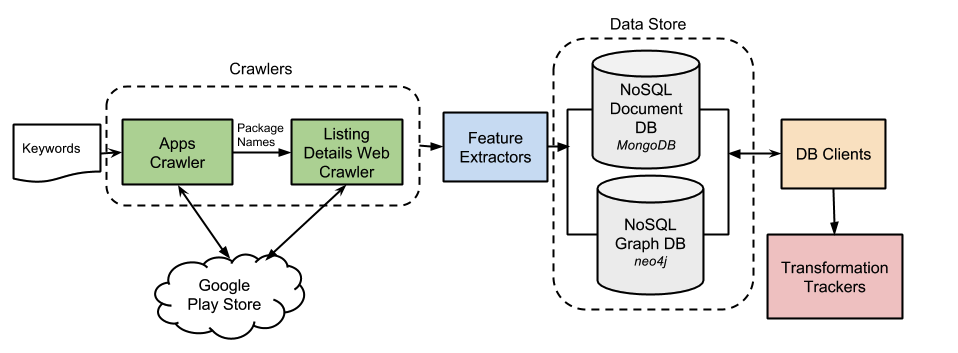
\includegraphics[width=16cm, height=5cm]{figures/design-pattern-changes/system_architecture}
	\caption{Architecture of the analytic system.}
	\label{fig:fig_system_architecture}
\end{figure*}

\begin{table*}[!t]
	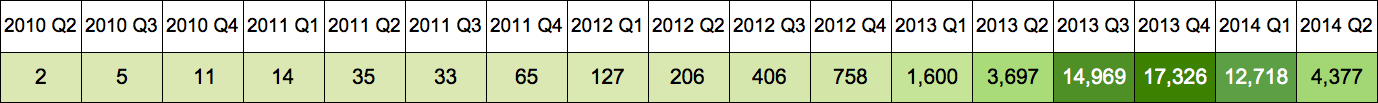
\includegraphics[width=16cm, height=2cm]{figures/design-pattern-changes/release_date}
	\caption{The number of apps by release date grouped by quarters.}
	\label{tbl:release_date}
\end{table*}

\par The system consists of five components (see Figure~\ref{fig:fig_system_architecture}): Apps crawlers, feature extractors, data stores, client drivers, and transformation (changes) trackers.
The apps crawler downloads free apps from the Google Play Store and saves them to the file system.
Feature extractors are a rich tool chain that decodes apps, extracts features, and stores them in the data stores.
The client drivers handle all interaction with the data stores.
The change trackers are a rich tool chain that tracks and computes statistics on changes to the extracted features.

\subsection{Apps Crawlers}
Our system utilizes two custom crawlers we built: the apps crawler and the listing details web crawler.
The apps crawler maintains a list of keywords, crawls the Google Play Store, and returns a list of package names for free apps.
We used Google-Play-Crawler \footnote{http://github.com/Akdeniz/google-play-crawler}, an unofficial open-source Java API for the Google Play Store, to retrieve package names and download APK files.
Prior releases of apps are not available on the Google Play Store.
Thus, the apps crawler obtains the version code value for each retrieved package name and queries the data store to check if it exists.
If it does not already exist in the repository, the crawler downloads and saves the APK file in the data store.

\par Once the APK file is downloaded, the apps crawler notifies the listing details web crawler to download the most recent app listing details web page.
The listing details web crawler is written in Ruby.
It generates a URL using the package name and downloads both the HTML page and the resources of the listing details web page.
Finally, another process runs to decode the APK file using Apktool \cite{apktool}, an open-source reverse-engineering tool.
When the APK file is decoded, we get a directory tree of app files that make up the app.

\subsection{Feature Extractors}
Once an APK file and its listing details web page have been downloaded, a set of feature extractors is run.
The feature extractors comprise three main tools: Listing details extractor, UI extractor, and source code extractor.
The listing details extractor parses the listing details HTML file, extracts the features, and stores them in the document data store.
The UI extractor traverses the unpacked APK file, extracts UI features from layout files and resources, and stores them in the graph data store.
The source code extractor computes features from the smali files, a human readable assembly like language for the disassembled byte code.
It uses string pattern matching techniques (e.g., grep, regular expressions) to extract features available in the app's byte code and stores them in the document data store.

\subsection{Data Stores}
Our data store is built on top of two database technologies: a NoSQL document-oriented database for storing apps listing detail features, code features, and APK files.
The second database is a graph database for storing the XML elements of layout files. The document-oriented database is a MongoDB instance, an open-source document- oriented database scalable to accommodate large and complex data. Our MongoDB instance comprises five collections: listing details, the AndroidManifest features, code features, and two GridFS collections to store the binary APK files and additional metadata. The MongoDB instance contains collections for over 56,349 APK files for 24,436 unique apps with multiple releases. The total size of the database is 501 GB hosted on a 24-core server with 47 GB RAM running Ubuntu 12.04. Over the observation period of our analysis (from January 2013 to June 2014), we collected a minimum number of versions per app in two versions in our dataset, which represents 80.1\% of the dataset (Figure~\ref{fig:fig_dataset}). Table~\ref{tbl:release_date} shows the number of apps by release date, and Figure~\ref{fig:fig_downloads_ratings} shows the download count distribution by their ratings.
\begin{figure}
	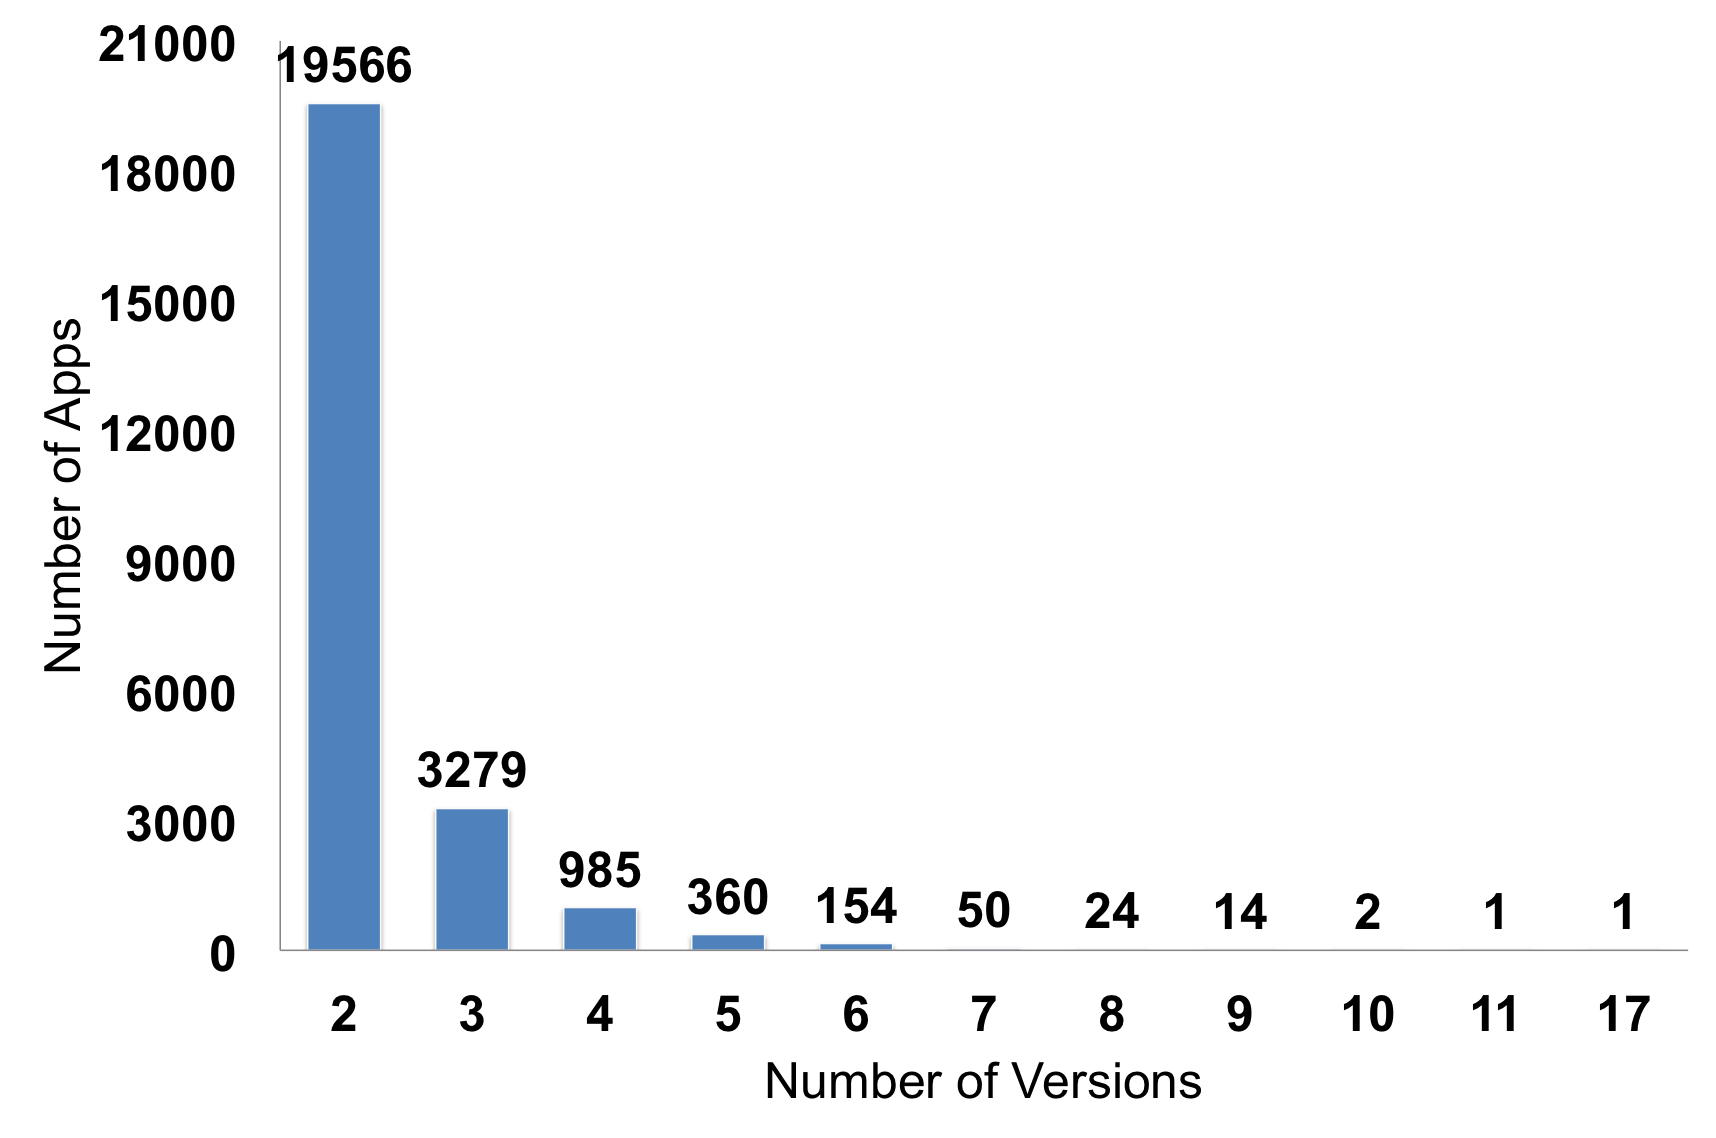
\includegraphics[width=6in, height=3in]{figures/design-pattern-changes/dataset}
	\caption{The distribution of apps by versions.}
	\label{fig:fig_dataset}
\end{figure}


\begin{figure*}[!t]
	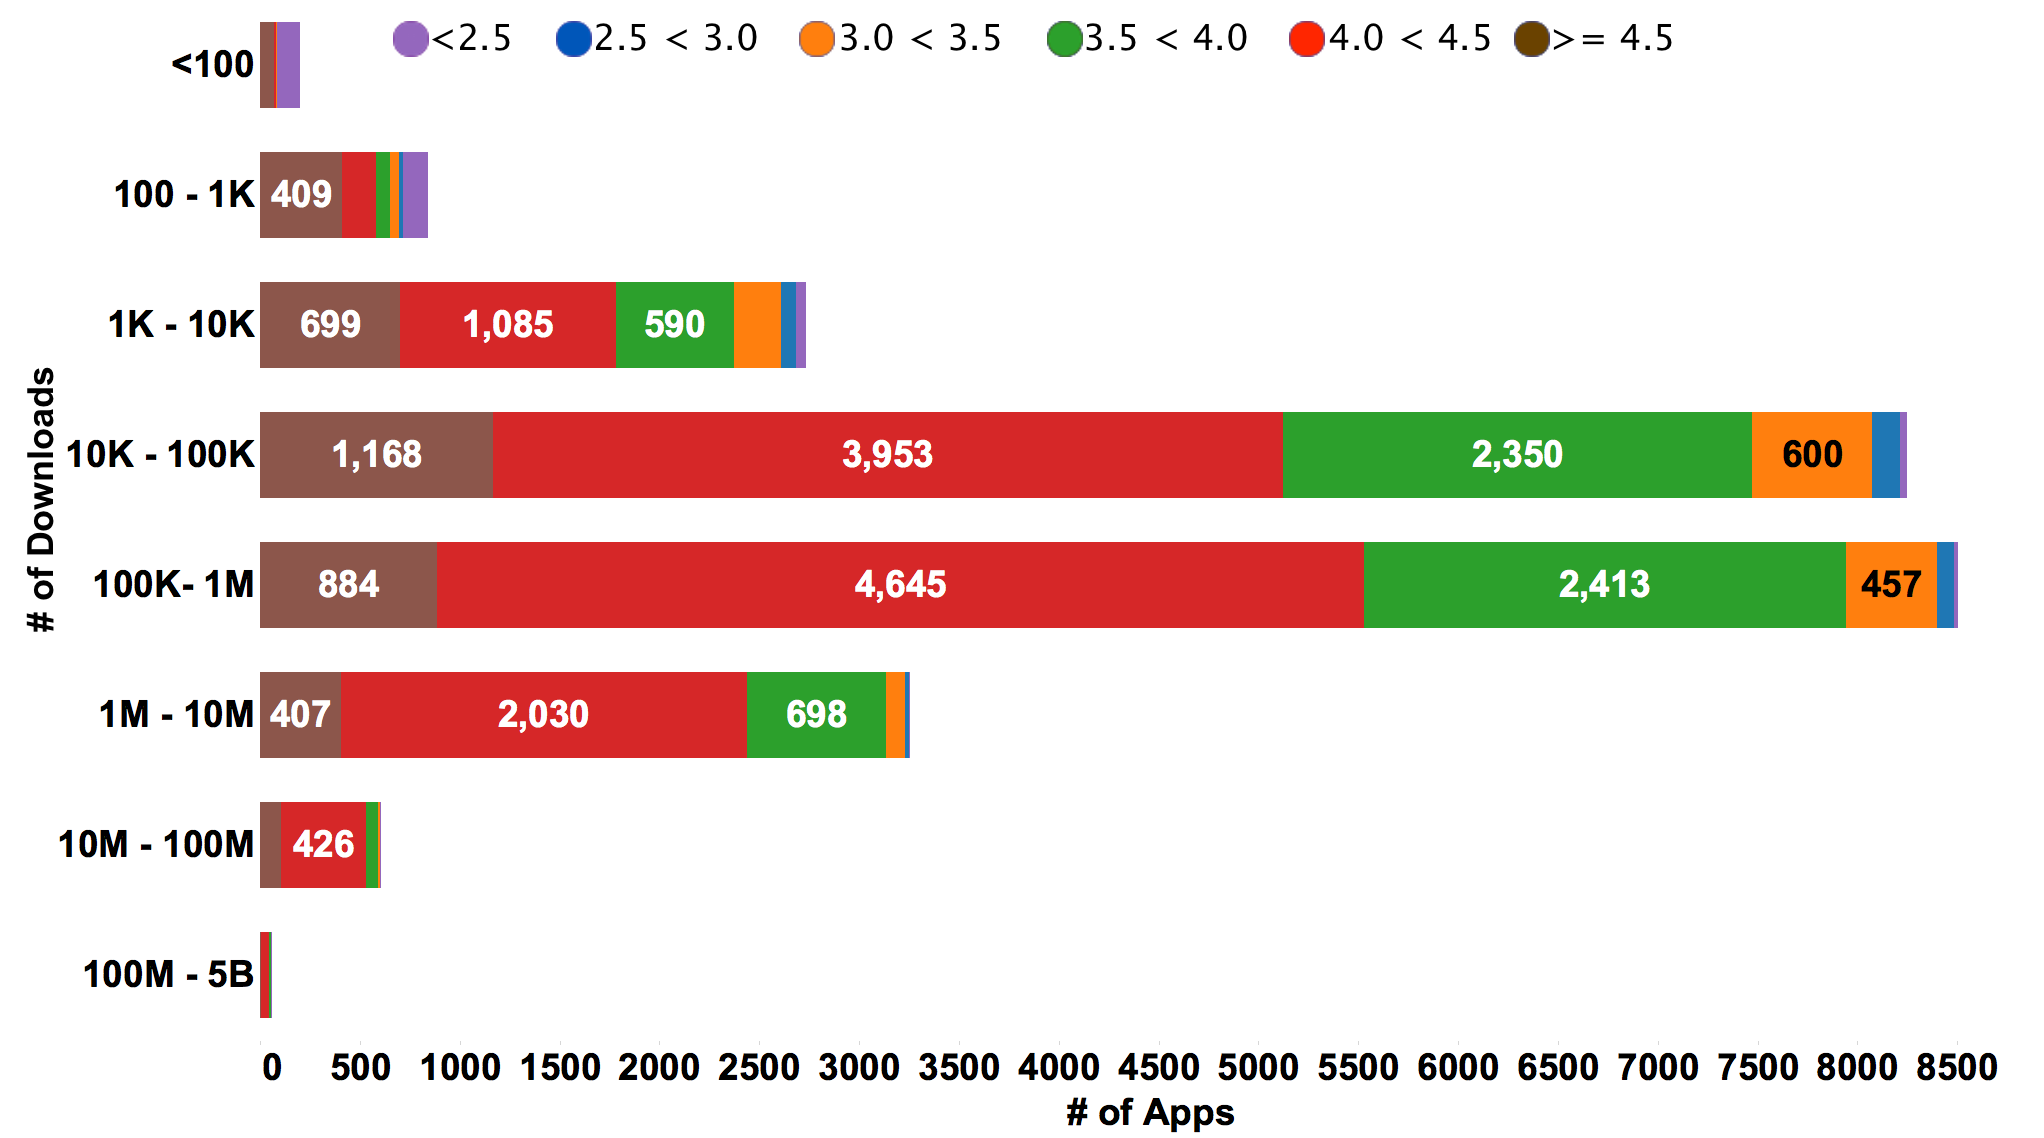
\includegraphics[width=16.5cm, height=8cm]{figures/design-pattern-changes/downloads_ratings}
	\caption{The download distribution of the apps by rating stars. Colors show details about the rating.}
	\label{fig:fig_downloads_ratings}
\end{figure*}

\par
The graph database is a Neo4j server. Graph databases are well suited to model hierarchical connected data like UI structure.
Neo4j uses the property-graph model, which allows storing XML elements with their attributes (key-value-pairs) in graph nodes.
In android, developers can reuse multiple layouts using the ``\textless include \textgreater '' tag to embed layouts to the current element in the hierarchy.
Our UI feature extractors attach the included layout to the current UI tree element, connecting layouts to one app tree.
Queries like ``find a specific ViewGroup element with two specific children'' run faster than the traditional many JOIN queries in Relational DBs.
In our database model, each UI element (e.g., a view like ImageView or a view group 
like LinearLayout) corresponds to a graph node connected with one relationship (e.g., has view, has view group).
The number of graph nodes in our database is 29,733,591 nodes.

\subsection{Database Client Drivers}
A set of MongoDB drivers is running to query and retrieve data from the database.
The complexity of the executed queries varies from finding fields in multiple collections to running multiple-pass mapReduce tasks.
The graph database clients execute transaction queries on the graph database using Cypher language, a graph query language for querying Neo4j graphs.
These clients output the results as CSV files to be processed by the transformation trackers.

\subsection{Transformation Trackers}

To interpret the results generated by the client drivers, another set of tools are running to compute statistics on the generated results.
These are data analysis tools written in Python using the Pandas library, an open-source library for high-performance data analysis.
The data store client drivers output the results as CSV files, which are passed as input to the transformation trackers.
The transformation trackers load each CSV file into a Data Frame, a tabular data structure with labeled axes.
The Data Frame is indexed by an array of tuples where each tuple is a unique value of the app's package name and version code values.
This makes it easier to track changes and perform sophisticated data analysis on multiple versions.

\section{Design Pattern Changes}
The system we developed has enabled us to conduct many analyses on design pattern changes.
Here we chose eight of the most illustrative ones to present: custom UI components, home screen widgets, as well as various ways of navigating: Tab Layouts, Fragments, Horizontal Paging, Action Bar with Tabs, Up Navigation, and Navigation Drawers. 
For each analysis, we discuss the motivation, method, results, and implications.

\subsection{Custom UI Components}

\subsubsection{Motivation}

A GUI framework typically provides a rich set of standard UI widget classes with the goal to ease the GUI development effort.
Developers often can meet their needs using these widget classes. 
If not, they may need to define custom UI widget classes. 
Some custom components are provided by third-party libraries to provide custom widgets or backward-compatibility of the standard components. 
Others are developer-customized components. 
How prevalent is the use of custom widgets? We are interested in this question because extensive uses of custom widgets may be a sign that the standard UI widget classes are inadequate.
\subsubsection{Method}
A custom component is declared in layout files using the full qualified class name of the component's class file which starts with a package name, such as
\begin{minted}{xml}
<com.android.notepad.MyEditText id="@+id/note" />
\end{minted}
rather than using the name of one of the default widget classes such as EditText, TextView, and Button.
Thus, to find evidence of use of custom UI components in an app, we queried the graph database for apps with views that start with a package name and counted the number of declarations of this form in all of the app's layout files.

\subsubsection{Results}

We found 15,808 (64.7\%) apps used at least one custom component, which is more than half of the apps in our corpus. 
Among them, 818 (5.2\%) apps initially did not use any custom component and began using it after an update. 
410 (2.6\%) apps did the opposite, reverting to use only standard components in subsequent updates. 
We looked at the listing details of these apps to find if the developers described any information related to this change in the listing details section ``What's New''.
We searched for UI related keywords and discovered apps that report enhancements to tablets and large screens.
For example, one app stated, ``App is optimized for tablets and many UI enhancements'' and another app stated ``Improved layout and graphics for larger screen''.
We also looked for unusual change patterns.
For example, we were interested in whether there were apps that had introduced a large number of custom components after an update.
We found 58 apps added more than 500 custom components after updates. 
We identified  234 unique custom components in these apps by the first three parts of the custom component name (e.g., com.airbnb.android).
The top three added custom libraries are: android.support.v4 (18.8\%), com.facebook.widget (11.5\%), and com.actionbarsherlock (5.1\%).
Interestingly, we observed a high concentration of these apps in the Finance category.
To dig further, we examined the ``what's new'' section of these apps and found mentions of ``tablets'' and ``large screens'' that coincide with this sudden increase in the use of custom components.
For example, one app stated ``Accept payment on Tablets'' and another one stated ``Resolved login crashes on multiple Tablets.''

\subsubsection{Discussion}

Even though most of the standard Android UI components provide built-in support for automatic scaling to fit content on large screens, getting these components to work properly may require a tremendous amount of effort by developers.
We speculate that the 818 (5.2\%) apps we found that had begun to use custom components may be to achieve better large screen support that is not offered by standard components.
We found there were more apps adding custom components than those removing custom components.
This suggests an increased level of reliance on custom components over our sample of Android apps.
One could interpret this as a sign that default components are gradually becoming inadequate.

\subsection{Home Screen Widgets}

\subsubsection{Motivation}

Home screen widgets are shown on the user's home screen to provide immediate access to useful information (e.g., today's weather) or control of commonly used functionalities (skipping to the next song).
By choosing which app's home screen widget to display, a user may implicitly indicate her preference for the app. 
Since there is limited area on the home screen, the size of a home screen widget matters. 
An app widget may provide a set of predefined dimensions (e.g., 1x1 or 2x2). 
Some apps may allow the users to adjust or stretch the dimensions of its home screen widgets freely.

\subsubsection{Method}

To find apps that use widgets, we queried the document database for apps that declare widgets in the app’s AndroidManifest.xml file. 
In this file, the \textit{\textless receiver\textgreater} element has a child element named \textit{\textless meta-data\textgreater} that has an attribute named \textit{android:name} whose value is set to \textit{``android.appwidget.provider''}. 
To support resizable widgets, Android developers need to declare the resize mode to be horizontal, vertical, or both by setting the value of the attribute \textit{resizeMode} of the \textit{\textless appwidget-provider\textgreater} element located at \textit{res/xml/}. 
To find resizable widgets, we queried the UI graph database to a find a widget layout file whose root element is \textit{\textless appwidget-provider\textgreater} with the attribute \textit{resizeMode}.

\subsubsection{Results}

We found 2,639 apps (10.8\%) support home widgets.
Among them, 255 (9.6\%) added home widgets for the first time, and 80 (3\%) later dropped home widgets altogether. 
1,118 (42\%) apps allow home widgets to be resizable. 
Among these, 295 (26.4\%) were not resizable before and became resizable only in the most recent release. 
24 (2.1\%) apps had resizable home screen widgets but later on disabled the resizing functionality. 
In all cases, we did not find any information in the listing (i.e., description and what's new sections) mentioning changes in home widget support. Figure~\ref{fig:fig_resizble_widgets}
\begin{figure}[!t]
	\centering
	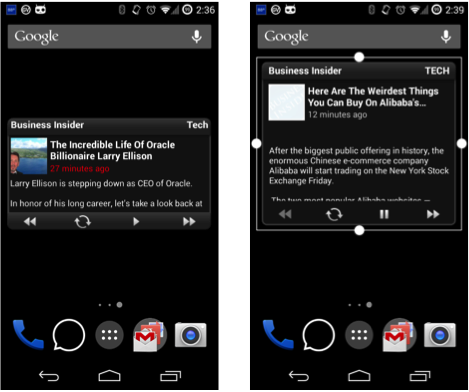
\includegraphics{figures/design-pattern-changes/resizble_widgets}
	\caption{Two versions of an app titled ``Business Insider'' before (left) and after (right) adding the resizing functionality to its home screen widget.}
	\label{fig:fig_resizble_widgets}
\end{figure}
shows an example of a home screen widget of an app before and after making it resizable.

\subsubsection{Discussion}

We found more apps adding support for home screen widgets than those dropping the support (255 vs. 80). 
This suggests an increased adoption of home screen design pattern. 
Among those already providing home screen widgets, a similar trend of increased adoption of the ``resizable'' pattern is observed. 
This suggests apps are increasingly competing for the limited home screen space. 
Apps that did not provide home screen widgets would lose out because users are unable to place them on their home screen and may use them less frequently as a result.

\subsection{Tab Layout with TabHost}

\subsubsection{Motivation}
Tab layouts are used to hold a set of tab labels to allow users to navigate between different content. 
One way to implement this design pattern is through the TabHost API. 
We chose this API for two reasons. 
First, this API was included in the initial release of the Android GUI framework (level 1). 
Second, it was later deprecated (level 11) in favor of new navigation patterns, such as the Fragment and the Action Bar patterns. 
We were interested in whether most or only a small percentage of apps had made this transition.

\subsubsection{Method}
In order to create a tabbed UI, developers need to use a ViewGroup element named TabHost and a View element named TabWidget. 
We queried the UI database for a GroupView named TabHost with a child View named TabWidget.
\subsubsection{Results}
We found 3,809 (15.6\%) apps used TabHost in their UIs. 
Among them, 666 (17.5\%) apps used TabHost for the first time and 413 (10.8\%) apps stopped using it and shifted to other types of navigations. 
We further inspected their listing details to see if it includes reasons that describe the migration. 
We found 106 (25.58\%) of these apps provided explanations in their listings. 
DDLive is an example of an app that has undergone this change. 
In the ``what's new'' section of its listing on Google Play, the phrase ``UI Changes for better experience'' can be found. 
Figure~\ref{fig:fig_tabhost}
\begin{figure}[!t]
	\centering
	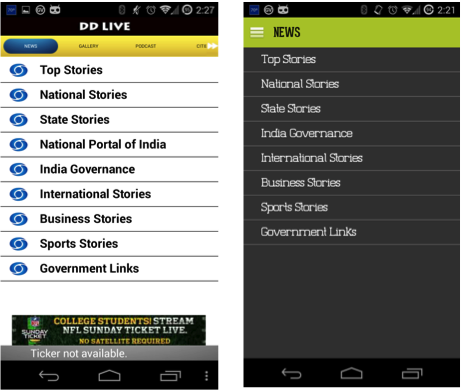
\includegraphics{figures/design-pattern-changes/tabhost}
	\caption{Two versions of an app titled ``DDLive''. The version on the left uses TabHost and the version on the right uses a Fragment that contains a list of items.}
	\label{fig:fig_tabhost}
\end{figure}
shows two screenshots of the app before and after the migration from the TabHost pattern to the Fragment pattern.

\subsubsection{Discussion}
The migration rate of this design pattern is very slow. 
Even though the TabHost pattern has been deprecated for at least three years, some new apps continued to use it. 
Existing apps using them slowly dropped the use of the TabHost pattern but not at a very fast rate. 
This raises the question of why deprecated APIs and design patterns enabled by them are so ``sticky'' among Android apps.

\subsection{Fragment}

\subsubsection{Motivation}
Fragments are used to create a multi-pane view and a responsive UI that works on a variety of screen sizes and devices. 
It is a relatively new design pattern that was introduced in API level 11 to allow developers to add multiple independent UI components and reuse them in different parts of the UI with its own lifecycle. 
We were interested in how widely this design pattern was adopted.

\subsubsection{Method}
Fragments can be statically added to the layout files or dynamically added in the source code. 
Thus, our analysis needs to look at both the UI and code. 
In the UI, we query the UI database for apps with the \textit{\textless fragment \textgreater} element and obtain the value of the \textit{android:name} attribute that references a class in the source code. 
In the code, we search for the class to see if it extends the Fragment class or any of its subclasses.

\subsubsection{Results}
We found 3,963 (16.2\%) apps used the Fragments pattern. 
Among them, 1,814 (45.8\%) used Fragment for the first time and only 139 (3.5\%) apps stopped using it in recent releases. 
Figure~\ref{fig:fig_fragment}
\begin{figure}[!t]
	\centering
	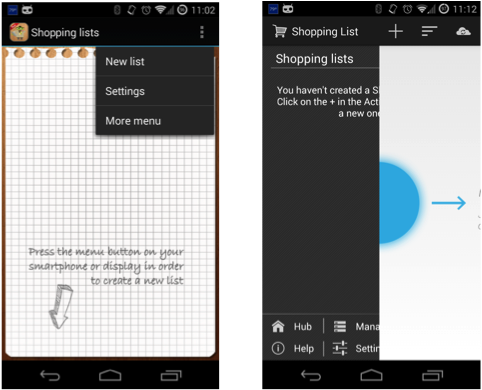
\includegraphics{figures/design-pattern-changes/fragment}
	\caption{Two versions of an app titled ``Shopping List'' before (left) and after (right) adopting the Fragment design pattern.}
	\label{fig:fig_fragment}
\end{figure}
shows an example of a shopping list app before and after using Fragment pattern.

\subsubsection{Discussion}
It had been four years since the Fragment pattern was introduced. 
We initially anticipated to observe a broad adoption of the Fragment pattern by apps to take advantage of the benefit this pattern offers. 
We instead found a lower than expected adoption rate. 
Only 3,963 (16.2\%) of the apps use it. 
Among them, almost half were recent adoption during our observation period. 
We speculate that the Fragment pattern is a lot more complicated to implement. 
For example,  StackOverflow, a popular online community for developers to ask and answer questions about coding, has over 16,100 questions tagged with ``android-fragments''. 
Some developers may rather stick to what they are familiar with rather than risking implementing the switch to the Fragment pattern incorrectly.

\subsection{Horizontal Paging}

\subsubsection{Motivation}
Horizontal paging is a navigation pattern that allows users to navigate between screens using left and right swipes. 
We explore this design pattern to find how wide this type of interaction is and how preferable it is over multiple releases.
\\
\subsubsection{Method}
To implement this pattern, the most common approach is to use a \textit{ViewPager} view group, which is a container that can hold multiple child view elements, each of which represents a distinct screen. 
Child views can be populated using \textit{PagerAdapters} in the source code. 
To find apps with this pattern, we queried the UI graph database for apps that use the \textit{ViewPager} element as a \textit{ViewGroup} container and make use of any \textit{PagerAdapters} subclasses in the source code.

\subsubsection{Results}
We found 4,524 (18.51\%) apps used the Horizontal Paging pattern. 
Among them, 941 (20.8\%) added this pattern for the first time. 149 (3.3\%) apps dropped this pattern. 
Figure~\ref{fig:fig_horizontal_paging}
\begin{figure}[!t]
	\centering
	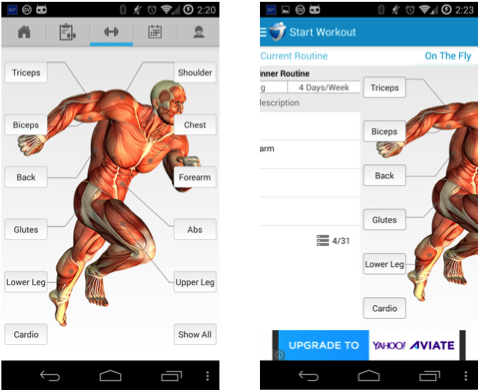
\includegraphics{figures/design-pattern-changes/horizontalpaging}
	\caption{Example of an app titled ``JEFIT Workout Exercise Trainer'' before (left) and after (right) adopting the Horizontal Paging design pattern.}
	\label{fig:fig_horizontal_paging}
\end{figure}
shows an example of an app before and after using the horizontal paging design pattern.

\subsubsection{Discussion}
We observed a lower first-time adoption rate of the Horizontal Paging pattern than that of the Fragment pattern. 
This suggests that Horizontal Paging pattern has a longer history than the Fragment pattern. 
Apps still continue to migrate to these two patterns but more of them chose the more general Fragment pattern.

\subsection{Action Bar with Tabs}

\subsubsection{Motivation}
Action Bar provides several functions to an app including the screen title, action buttons, and a navigation view with two modes of navigations: navigation tabs or drop-down lists. 
It was first introduced in Android 3.0 (API level 11) but also available for lower API levels through additional support libraries. 
We explore the use of the Action Bar with navigation tabs, and how apps have maintained the use of this pattern in their recent versions.

\subsubsection{Method}
While there are multiple ways to create an Action Bar with navigation tabs, they all require implementing the \textit{ActionBar.TabListener} interface that provides the required callbacks to respond to user's actions. 
To explore the use of Action Bar with tabs, our analysis needs to look at the code. 
We search the source code for apps that implement the \textit{TabListener} interface.

\subsubsection{Results}
We found 8,483 (34.7\%) apps used the Action Bar with Tabs. 
Among them, 2,729 (32.2\%) were first-time adopters of this pattern. 330 (3.9\%) stopped using it. Figure~\ref{fig:fig_actiobar_tabs}
\begin{figure}[!t]
	\centering
	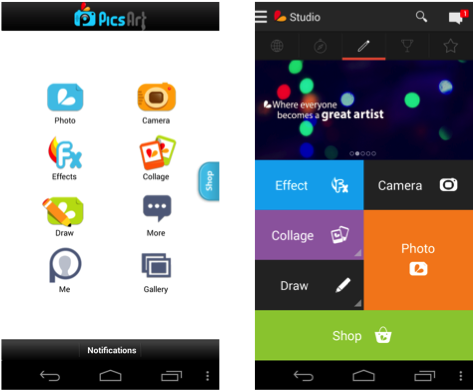
\includegraphics{figures/design-pattern-changes/actiobar_tabs}
	\caption{Two versions of an app titled ``PicsArt'' before (left) and after (right) adopting the Action Bar pattern with Tabs.}
	\label{fig:fig_actiobar_tabs}
\end{figure}
shows an example of an app before and after using the Action Bar with Tabs.

\subsubsection{Discussion}
The Action bar with navigation tabs design pattern is the most commonly used new navigation design pattern in our dataset of apps. 
34.7\% of the apps used it. 
We suspect the reason is that this pattern has been considered mainstream over the past couple years. 
An app would look out of date without adopting this pattern. 
Moreover, the Action Bar API is one of the easier APIs for developers to implement and add additional functionalities such as title, icon, and view controls. 
Yet, 330 still decided to remove the Action Bar pattern.

\subsection{Up Navigation}

\subsubsection{Motivation}
Apps can use the app icon as an Up button to support navigation between screens based on their hierarchal relationships. 
We study the use of this pattern because it provides a new way of navigation based on the app's hierarchy rather than navigating through the history of visited screens, a feature already provided by the physical Back button. 
Unlike the physical Back button, the Up button always ensures that the user navigates through the parent of the current screen and does not exit the app while navigation. 
The Up button usually appears as a left-facing caret to the left of the app icon in the \textit{Action Bar}. 
When a user taps on the Up button, the app navigates to the parent screen in the activity hierarchy.

\subsubsection{Method}
In order to use Up buttons, developers need to call the \textit{setDisplayHomeAsUpEnabled} of the \textit{ActionBar} class. 
To find this navigation mechanism, our analysis searches the app's code for the fully qualified name of this method.

\subsubsection{Results}
We found 4,431 apps (18\%) used this navigation pattern. 
Among them, 1,257 (28.4\%) added it for the first time and only 98 (2.2\%) of the app's stopped using it. 
Figure~\ref{fig:fig_upnav}
\begin{figure}[!t]
	\centering
	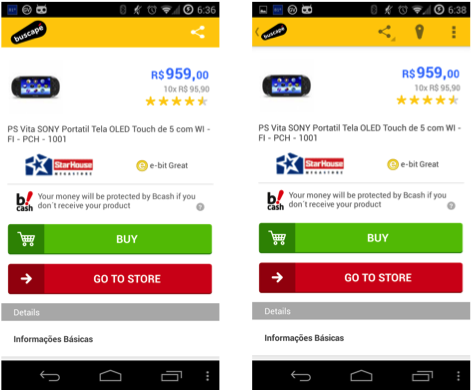
\includegraphics{figures/design-pattern-changes/upnav}
	\caption{Two versions of an app titled ``Buscape'' before (left) and after (right) adopting the Up Navigation pattern. The Up navigation button is shown at the top left corner as a left-facing caret next to the app icon.}
	\label{fig:fig_upnav}
\end{figure}
shows an example of an app before and after using it.

\subsubsection{Discussion}
The Up navigation pattern is less common than navigating with a physical back button. Only 18\% of the apps adopt this pattern. 
The reason behind the Up navigation pattern's low adoption rate could be that apps have relied on the back button for navigation since the initial release of Android, which is already implemented by default. 
The Up navigation button was common in apps that have several sibling activities in the hierarchy (e.g., email clients, shopping apps), which may not be the case for most apps.

\subsection{Navigation Drawers}
\subsubsection{Motivation}
Navigation Drawer is a hidden panel that displays the app's main navigation menu. 
It helps users quickly navigate through the structure of the app. 
When the user taps on the top-left app's icon or swipes from the left to the right of the screen, the Navigation Drawer expands to cover part of the screen and shows a list of items.

\subsubsection{Method}
In order to use the Navigation Drawer, developers need to create a layout with a \textit{DrawerLayout} as the root \textit{ViewGroup} element with two children elements. 
The first child is the Layout element that represents the content when the drawer is hidden and the second is the actual drawer that slides in the Navigation Drawer panel. 
We queried the graph database to find apps that have layouts that starts with a \textit{DrawerLayout} element as a root element with two child views.
\subsubsection{Results}
We found 1,183 apps used the Navigation Drawer. 
Among them, 771 (65.2\%) added it for the first time and only 37 (3.1\%) of the apps stopped using this pattern. Figure~\ref{fig:fig_drawer} shows an example of an app before and after using this pattern.
\begin{figure}[!t]
	\centering
	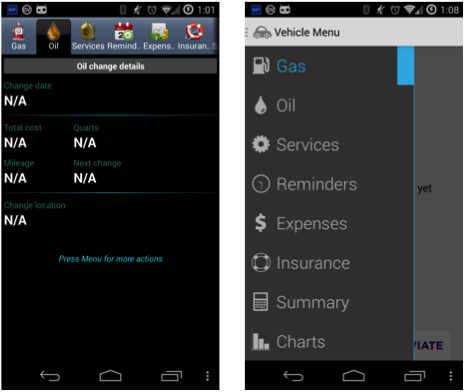
\includegraphics{figures/design-pattern-changes/drawer}
	\caption{Example of an app titled ``Carango - Car Management'' that shows two versions before (left) and after (right) using the Navigation Drawer pattern.}
	\label{fig:fig_drawer}
\end{figure}
\subsubsection{Discussion}
Navigation drawer is relatively less common than other navigation patterns. 
We speculate the reason is two-folds. 
First, implementing this pattern requires a high degree of customization by developers to fit their needs. Second, an app may not have a deep hierarchical navigation structure to make use of this pattern. 
We also found that the majority of the apps using the Navigation Drawer were recent adopters (771 out of 1183), which suggests Navigation Drawer a relatively new design pattern.

\section{Summary}
This chapter presented a large-scale data-mining approach to analyzing design pattern changes.
I discussed its implementation and illustrated a subset of analyses regarding the changes in the use of design patterns (see table~\ref{tab:table_summary}).
This work demonstrated the value of using data-driven approaches to discovering design pattern changes on a large-scale.

\begin{table}[!htbp]
	\def\arraystretch{2}
	\begin{tabular}{| >{\centering\arraybackslash}m{6cm} | m{2cm} | m{2cm} | m{2cm} | m{2cm} |}
		\hline
		\centering Design Pattern & Usage & First \ Time & Changes & No Changes \\
		\hline
		Custom \ UI \ Components & 15,808 & 818 & 410 & 15,398 \tabularnewline
		\hline
		Home Screen Widgets & 2,639 & 255 & 80 & 2,559 \tabularnewline
		\hline
		Resizable Home Screen Widgets & 1,118 & 295 & 24 & 1,094 \tabularnewline
		\hline
		Tab Layout with TabHost & 3,809 & 666 & 413 & 3,396 \tabularnewline
		\hline
		Fragment & 3,963 & 1,814 & 139 & 3,824 \tabularnewline
		\hline
		Horizontal Paging & 4,524 & 941 & 149 & 4,375 \tabularnewline
		\hline
		Action Bar with Tabs & 8,483 & 2,729 & 330 & 8,153 \tabularnewline
		\hline
		Up Navigation & 4,431 & 1,257 & 98 & 4,333 \tabularnewline
		\hline
		Navigation Drawers & 1,183 & 771 & 37 & 11,46 \tabularnewline
		\hline
	\end{tabular}
	\caption{The changes to the presented design patterns. The columns show the name of the design pattern, the number of apps that used this pattern in the dataset, the number of apps that used it for the first time in a recent release, the number of apps that used it but later switched to a different design pattern, and the number of apps that maintained using it in future releases.}
	\label{tab:table_summary}
\end{table}
\chapter{Sieveable: A Scalable Platform for Mining Mobile Applications}
\label{ch:sieveable_chapter}
As the number of mobile apps continue to proliferate in marketplaces, the need to study them at large-scale has begun to receive increased attention. 
Most of the prior work in this area is limited to a single view of the data  and lacks a  holistic view of the apps. 
In addition, data-driven systems are largely constrained by the availability of samples and efficient indexing.
This chapter presents Sieveable, a multi-view search engine for Android apps.
Sieveable enables deep searching and filtering across multiple levels: (a) Listing Details, (b) User Interface structure, (c) Manifest structure, and (d) API calls. 
Sieveable crawled and indexed more than 450,000 apps.
It provides a query by example language to specify deep search queries.
I discuss the key challenges in designing and developing a scalable retrieval system to enable the deep and longitudinal approach presented in this dissertation.

\section{Introduction}
Mobile software platforms feature a distribution platform for applications called marketplaces (or app stores).
App marketplaces have become the largest platform for distributing mobile applications, where users can search for apps, browse through different categories, rate or review apps, and install free and paid apps.
The popularity of mobile devices and the advances in their operating systems have led to a significant increase in the number of apps published in marketplaces.
For example, as of April 2016, the number of apps in the Google Play Store has exceeded two million apps \cite{appbrain_play_apps}.
These apps have become a valuable data source to mine and extract insight from in both academia and industry.

In the recent years, there has been a noticeable amount of research activities on how to extract meaningful insights from apps data.
The research in mining mobile apps has been dominated by three single views.
First, researchers have mined the listing details data (metadata) of apps such as ratings and user reviews to perform sentiment analysis and help developers make informed decisions supported by data \cite{fu_2013_KDD,chen_2014_ICSE,kong_2015_CCS}. 
Others have created tools and commercial services to assist app developers and publishers in better understanding of listing details data \cite{appfigures,applause,appannie}.
Second, researchers have mined user interface (UI) design data such as styles and layouts of thousands of apps to gain insights into their design patterns \cite{shirazi_EICS_2013} and my work in chapter~\ref{ch:mining_design_changes_chapter}.
Third researchers have also mined the source code of apps to learn about malicious behavior and protect users' privacy-sensitive data \cite{zhou_2012_SP_dissecting,lu_2012_CCS,Arzt_2014_PLDI}.
What is missing in prior research is an approach that takes both a holistic view (design and development) and temporal view (multiple versions) of the apps.
There are multiple benefits for considering a holistic view that involves both design and development views in mobile app analysis.

% Design and Development
App design analysis focuses on UI related data (e.g.,) layout and style files) while development analysis focuses on code and configuration data (e.g., Manifest files).
In design analysis, UI components are often created or modified at runtime.
When only analyzing the static layout files, this observation is missed because that behavior is defined in the app source code.
This shortcoming can be solved by combining both the design and development views.
In sentiment analysis of user reviews, it is often difficult to link opinions to specific features.
By incorporating the design view and development view, one can potentially establish a causal relationship between a new feature (or a bug) and the onset of certain opinions.
In security analysis, a function could be determined, through program analysis, to be triggering a sensitive operation, such as sending an SMS message or taking a photo.
But it is often hard to judge if the sensitive operation is warranted from the program view alone.
By also taking a view of the design, one may examine which button may be linked to this sensitive operation and whether the button's label legitimizes such use: for example, ``Send'' for sending an SMS message.
% Temporal analysis
Furthermore, the increase number of app updates published to marketplaces has largely gone unobserved. 
By only considering a single version of the app, one cannot form a deep understanding of the emerging trends in mobile design and development.
% Scalable
Supporting multi-view temporal analysis of apps is always challenging because it requires a scalable infrastructure for integrating multiple heterogeneous data sources.
The store listing details data is document-oriented where every app shares a number of common fields such as the title, ratings, and category, which can be mined from app marketplaces.
Design data is hierarchical; the layout files specify the relationship between various UI components in a tree structure.
Program data is highly structural as it involves a large number of names of classes, methods, and variables.
Mining apps in multiple views would require an integrated infrastructure that supports document-oriented, hierarchical, and structural data, and provides an easy interface to store, index, mine and analyze such data.

In this chapter, I pursues a more general analysis approach that takes a holistic view of the apps over time and can potentially accomplish what is currently not possible in a single-view, single-version approach.
I present \emph{Sieveable}, a novel retrieval platform for multi-view data mining of apps on a large scale to address the needs mentioned above.
I discuss a new query language with a declarative, ``example-based'' syntax.
Using this language, analysts could quickly retrieve a sample from a large corpus of apps that meet certain criteria with respect to the listing view, design view, and program view in an integrated manner.
Prior to Sieveable, each of these analyses would take days of effort in writing custom scripts and running them on a cluster of servers (my work in chapter~\ref{ch:mining_design_changes_chapter}).
With Sieveable, each analysis task can be expressed as a search query and results can be obtained in a matter of minutes.
The chapter continues as follows. An overview of our system, detail description of its implementation to enable a new multi-view analytical queries.


\section{System Overview}
In this section, we describe the key requirements of our system and its core components at a high level.

\begin{table*}[t]
	\def\arraystretch{2}
	\centering
	\begin{tabular}{|>{\raggedright}p{2cm}|p{12.5cm}|}
		\hline
		\textbf{Listing \ Details \ Features} &
		package name, title, description, reviews, store URL, category, price, date published, version name, version code, target system version, ratings count, rating, content rating, creator, creator URL, install size, downloads count, permissions, what's new.\\
		\hline
		\textbf{User Interface Features} &
		layout directories, XML layout file DOM structure, drawable resources, string resources.\\
		\hline
		\textbf{Manifest Features}&
		Manifest File XML DOM structure, which includes elements such as activities, permissions, services, etc.\\
		\hline
		\textbf{Code \ Features} & 
		Framework API invocations, dependency libraries.\\
		\hline
	\end{tabular}
	\caption{Sieveable's main extracted features.}
	\label{tab:table_features}
\end{table*}

\subsection{Requirements}
We identify four main requirements that drive the technical development of the our system:
\begin{itemize}
	\item \textbf{Generalizable:}
	Given the large and diverse ecosystem of the Android platform, our search engine must be general enough to meet diverse user search goals.
	One may use the system to search for user interface design examples, API usage examples, or security permissions that protect sensitive resources.
	In order to meet various search goals, Sieveable captures powerful app's features and uses an example-based search.
	
	\item \textbf{Scalable:}
	Given the large volume of apps updated frequently, it is essential to design a scalable search engine.
	The system must be designed to be highly scalable to index billions of files. We address this goal by building a distributed search engine that can be scaled horizontally when an index becomes too large to fit a single machine.
	\item \textbf{Deep:}
	The search must be comprehensive and deep, taking into account features intrinsic to the app, such as code and UI data, as well as extrinsic features that describe the app, such as the marketplace listing details information.
	
	\item \textbf{Extensible:}
	The system must be designed to be modular and extensible to easily extend its search capabilities.
	To achieve this goal, Sieveable uses a modular plug-in architecture where each search level (e.g., UI search, code search) is a separate module that can be incorporated to the search system.
	By delegating search tasks into modules, a developer may add a new plug-in to extend the search system.
	For example, a developer may create a search plug-in for finding open source Android apps hosted on GitHub.
\end{itemize}

\subsection{Approach}
We present a novel approach that supports searching apps across multiple levels.
Our approach consists of four main steps: data collection, features extraction, features indexing, and a language specification for performing search queries.

\subsubsection{Data Collection}
We download the Android Application Package (APK) file for apps from the official marketplace, Google Play Store.
For each APK file we download and add to the dataset, a web crawler is run to obtain its listing details web page.
Next, we parsed the listing details HTML page to extract store listing values.
In order to expose the app's UI and code structure, we run a reverse-engineering tool to decompile it, which results in a directory tree of app files that make up the app. 
With more than one year effort, we manged to collect 452,775 apps with multiple versions\footnote{Note that sometimes the crawler was down, so it may have missed a number of updates.}.

\subsubsection{Features Extraction}
Once an app is downloaded and decoded, we run a set of tools to extract features at four levels:
a) Listing details level: it includes information defined in the app's marketplace listing web page.
b) User interface level: it includes all layout related files.
c) Manifest level: it includes additional internal information that describes the app.
d) Source code level: it includes all API calls invoked by the app.
All extracted features are listed in Table~\ref{tab:table_features}.

\subsubsection{Features Indexing}
When app features are extracted, we store and index them in scalable data stores to support efficient execution of search queries.
Sieveable comprises four main data collections: APK files, listing details, user interface, Manifest, and source code.
1) APK files: The binary APK files are saved on disk across multiple locations and their paths are stored in a document-oriented database along with their name and version values to facilitate quick retrieval.
2) Listing details features are stored in a document-oriented database.
We use text indices on specific fields (description, what's new section, reviews, and title).
3) User interface: we use a structural index that keeps track of all DOM elements' relationships (parent/child and ancestor/descendant).
4) Manifest features: we index DOM element names and their attribute values.
5) Code: we use a text index to support search of invoked API classes and methods.

\subsubsection{Query Language Specification}
\underline{\textbf{Query Syntax:}}
Sieveable uses a SQL-like declarative query syntax. The syntax is composed of three main clauses:
\begin{itemize}
	\item \textit{MATCH} The app to match. 
	\item \textit{WHERE} The search condition.
	\item \textit{RETURN} The results to return.
\end{itemize}
Example:
\begin{minted}{xml}
	MATCH app
	WHERE
	    <LinearLayout>
	       <Button/>
	    </LinearLayout>
	RETURN app
\end{minted}
The \textit{MATCH} clause defines the apps to match for the given search conditions.
The \textit{WHERE} clause defines specific search conditions. 
A search condition in its simplest form is an example of a single listing details field, UI element, manifest element, or an API call.
Multiple search conditions can be combined together allowing for a deep search across multiple levels.
The \textit{RETURN} clause defines the subset of fields to include in the results.
Multiple levels search conditions can be added to the \textit{WHERE} clause.
For example, a search query for apps developed by \textit{Google}, have a \textit{LinearLayout} with a child \textit{Button}, use the SEND\_SMS permission, and call the takePicture API call, will look like:
\begin{listing}[ht]
	\begin{minted}{xml}
	MATCH app(latest=true)
	WHERE
	<developer>Google Inc.</developer>
	<LinearLayout>
	   <Button/>
	</LinearLayout>
	<uses-permission android:name="android.permission.SEND_SMS"/>
	<code class="android.hardware.Camera" method="takePicture"/>
	RETURN app
	\end{minted}
	\caption{Sieveable query example.}
	\label{lst:query_example}
\end{listing}

\underline{\textbf{Query Parser}}
When a query is submitted to Sieveable, it parses the search condition parts to determine their query levels (listing, UI, manifest, and code).
Sieveable maintains a set of dictionaries to lookup and extract search condition parts by their levels.
In particular, it maintains three dictionaries: a predefined set of listing details fields, and a set of manifest XML elements, and a single XML element named code for code related queries.
If an XML element in the query condition is not defined in any of the dictionaries, we consider it as a UI search element.
For example, Sieveable interprets the query in Listing~\ref{lst:query_example} as follows.
It parses the \textit{WHERE} clause part and groups the query parts by their levels.
This results in four query parts: a) listing details query for the \texttt{<developer>} tag, b) manifest query for the \texttt{<uses-permissions>} tag, c) code query for the \texttt{<code>} tag, and UI query for the remaining elements (\texttt{<LinearLayout>} and its child).
Sieveable sends these query parts to the query executor.

\underline{\textbf{Query Executor}}
\begin{figure}
	\centering
	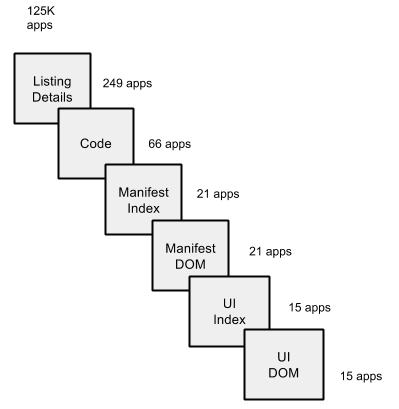
\includegraphics[scale=0.5]{figures/sieveable-deep-search/queryExecution}
	\caption{The execution sequence for a query that includes multiple level search conditions.}
	\label{fig:fig_query_execution}
\end{figure}
The query executor creates a plan for executing the received query parts.
The plan is an order of steps to query each index and data store (listing, UI, manifest, and code).
Query parts are executed by collection finder plug-ins (e.g., find by UI Index, find by UI DOM, find by code, etc.).
Collection finders return a set of app ids that matched the given query.
Sieveable computes the intersection of app ids to avoid scanning entire collections.
This also ensures that the final query results only contain ids for apps matched by all query conditions.

Figure~\ref{fig:fig_query_execution} shows the execution sequence of the query in Listing~\ref{lst:query_example} and the number of apps scanned by each collection.
The entire dataset contains over 400,000 apps.
The listing details query part is executed by the \textit{findByListing} module, which returns 249 apps developed by Google and filtered by the latest version of each app.
Next, the \textit{findByCode} module executes the code query part only on those 249 apps and returns 66 apps.
The \textit{findByManifestIndex} module searches the Manifest index for the Manifest query part only on those 66 apps and returns 21 apps.
The Manifest query part is sent to the \textit{findByManifestDOM} module to match the DOM tree for those 21 apps. Since the query part contains no hierarchical structure, the DOM matcher returns the 21 apps found by the index.
Next the UI query part is sent to the UI index to search for apps with LinearLayout and child Button.
The \textit{findByUIIndex} searches the UI index for those 21 apps  and finds that 15 of them have that UI structure.
The UI query part is sent to the \textit{findByUIDOM} module to match the DOM tree for those 15 apps which returns the final query results (15 apps).
Finally, Sieveable returns any field defined in the return clause for the matched app ids.
The return clause in the submitted query includes only a single app field, so Sieveable will return an array of objects where each object contains key-value pairs for the app id, package name, and version code. Below is part of the final query result:
\begin{minted}[fontsize=\footnotesize]{javascript}
[{ "app": { 
"id": "com.google.android.talk-21224130",
"packageName": "com.google.android.talk",
"version": "21224130"
}
}]
\end{minted}

\section{System Implementation}
\begin{figure*}[!t]
	\centering
	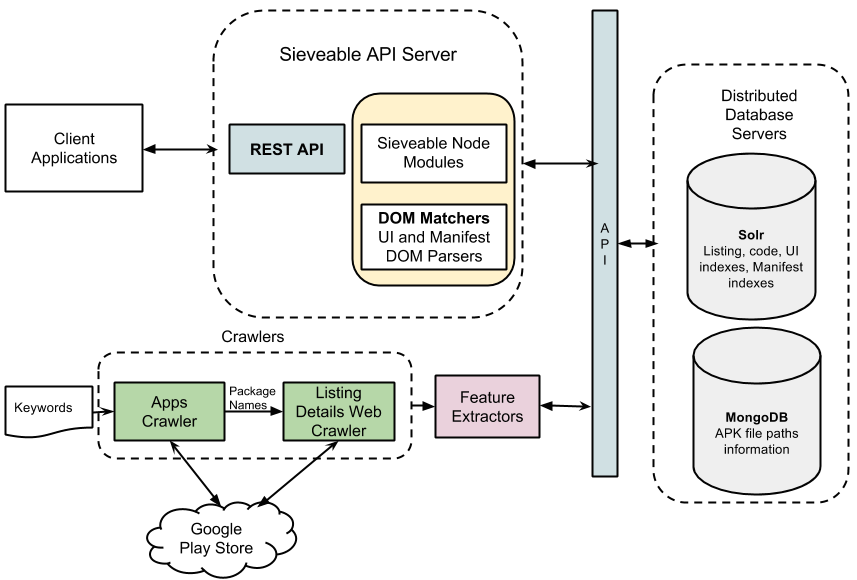
\includegraphics[width=17cm, height=10cm]{figures/sieveable-deep-search/architecture}
	\caption{Sieveable system architecture.}
	\label{fig:fig_architecture}
\end{figure*}

In this section, we discuss the technical details of designing and implementing our system. The system consists of six main components: app crawlers, feature extractors, data indexers, data store servers, DOM matchers, and a restful API (see Figure~\ref{fig:fig_architecture}).

\subsection{App Crawlers}
Sieveable features two crawlers that collect our dataset of apps: apps crawler and listing details web page crawler,
The app crawler is responsible for downloading APK files from the Google Play store.
We feed a dictionary of popular Android search keywords into the crawler.
Google has no official API for downloading APK files.
We used an unofficial API\footnote{http://github.com/Akdeniz/google-play-crawler} to collect APK files.
When an APK file is downloaded we run the Android Asset Packaging Tool (aapt) on the file to obtain its package name and version code.
We use a combination of the package name and version code as a unique identifier for each app.
APK files are stored in the file system while their ids and disk paths are stored in a MongoDB collection for fast retrieval.
Once an APK file is downloaded, we run a web crawler to fetch the most recent listing details web page of the app.
We parse the listing details fields and save them in another MongoDB collection.

\subsection{Feature Extractors}
We built a set of command line tools to extract features from the APK files.
First, we use apktool \cite{apktool}, an open-source reverse engineering tool, to decode the apps and obtain their source files.
Second, we run a custom UI parser that parses layout files and resolves any references to external resources (e.g., \texttt{android:text="@string/variable"}) or embedded layouts (using \texttt{<include/>} and \texttt{<merge/>} tags).
The parser produces a single XML file that contains the entire app UI tree, including all files.
This is especially important when performing DOM matching queries since it eliminates the need to load multiple layout files into memory when performing such queries.
Below is a snippet from an XML file generated for the YouTube app.

\begin{minted}{xml}
<App name="com.google.android.youtube" version_code="5021">
    <Directory directory_name="layout">
       <File file_name="activity_feed_item.xml">
          <RelativeLayout>
             <ImageView android:id="@id/channel_avatar"/>
           </RelativeLayout>
           ...
       </File>
    </Directory>
</App>
\end{minted}

Third, we extract all API calls from the smali files, a human readable assembly-like language for the disassembled byte code.
We save the extracted API calls in one text file per app.

\subsection{Data Indexers}
Sieveable indexes the extracted features in Solr collections for fast data access.
A collection is a complete logical index.
We use five Solr logical indexes to index our dataset: listing index, UI tag index, ui structural index, manifest tag index, and code index.

\textbf{Indexing Listing Details:} It contains all listing detail fields. Four fields are indexed as generic text fields (description, title, ``what's new'', and reviews) to support text based search.

\textbf{Indexing UI Data:} The extracted UI files are indexed in two Solr indices: \textit{1) Tag Index:} We extract all tag names and attributes and store them in one index document.
This index holds all tag names and their attributes.
\textit{2) Structural Index:} a suffix tree based index that stores the XML tree in a suffix array format \cite{shasha_2002_atreegrep}.
This index holds values that indicate the parent-child relationship of nodes in the XML tree. (e.g., \path{LinerLayout->Button}).
We parse the single XML UI tree file we extracted for each app and generate two text documents. The first text document contains the tag and attribute names for all UI elements (e.g., \path{EditText(android:layout_width="fill_parent")}).
We add this document to Solr and use it as the tag index.
The second generated document describes the UI tree in a suffix-tree format where each line corresponds to a root-to-leaf path for all XML elements (e.g., \path{RelativeLayout->LinearLayout->ImageButton}).
We add this document to Solr and use it as the structural index.

\textbf{Indexing Manifest Data:} The extracted manifest files are indexed by their tag names and attribute values.
Unlike UI queries, Manifest queries are less structural (e.g., find \path{"android.permission.CAMERA"}).
Therefore, we use the same UI tag index method to add manifest files to the Solr index.

\textbf{Indexing Code Files}, we add the extracted invoked API calls from the smali source code files to Solr.

\subsection{Data Store Servers}
Sieveable uses two main NoSQL database servers:
a) MongoDB \cite{mongodb}: is a document-oriented NoSQL database. It contains a collection for storing information about the downloaded APK files.
b) Apache Solr \cite{solr}: is a document-oriented NoSQL Search Platform.
We use Solr to store distributed collections for listing detail fields, UI tags and attributes, UI structural index, Manifest attributes, and code files.
Due to the large size of our data sets (over 8TB), we found that a single machine is not sufficient to store this large data sets.
Thus, we shard and replicate the collections across a cluster of multiple nodes to improve the system performance and availability.
We use an external Zookeeper \cite{zookeeper} cluster of five nodes to synchronize Solr's configuration and elect leaders.
\subsection{DOM Matchers}

Sieveable UI and Manifest search queries are written in  ``example-based'' syntax.
We implement a custom DOM matchers module to navigate the XML DOM tree and select DOM elements with a particular DOM structure.
The DOM matchers perform a jQuery like DOM manipulation.
While loading DOM files for complex queries is often considered expensive, the use of hierarchical indices reduce the number of false candidates significantly.
However, parsing the DOM for large number of files has an inevitable memory and system resources overhead.
Therefore, Sieveable uses a configurable default limit of 50 results per a given search query and return an inalterable cursor to the client to receive the entire query results.

\subsection{RESTful API}
Client applications can access Sieveable through a RESTful API.
The API provides an HTTP GET request mechanism allowing client applications to submit queries and receive the result as a JSON document.
For an easy query access, Sieveable has both a command line and web client applications that interact with the RESTful API.

\section{Summary}
This chapter presented Sieveable, a multi-view search engine for apps on a large-scale.
It discussed the importance of searching and mining apps across multiple views.
For the first time, Sieveable can help users execute deep search queries (illustrated in Chapter \ref{ch:findings_chapter}) and apply data driven approaches with a holistic view of apps at large-scale that could yield valuable results.
Sieveable has been deployed into a distributed computing infrastructure.
For more information on using Sieveable including source code access, please visit:
\url{http://github.com/sikuli/sieveable}.

\chapter{Deep Search Queries}
\label{ch:queries_chapter}

\section{Introduction}
Sieveable enables users to perform queries across multiple levels to meet diverse search goals.
It can find apps with specific listing fields, UI structures, manifest attributes, and API calls.
Sieveable can produce results beneficial to several stakeholder groups:
a) User interface design researchers can use Sieveable to find apps with specific design structures.
b) Accessibility researchers can use it to find answers to accessibility questions.
c) Privacy and security researchers can use it to find apps that request an unusual number of permissions or use vulnerable APIs.
d) Program analysts can use Sieveable to reduce the time to find examples of interest to apply defect analysis.
e) Data mining researchers can mine applications efficiently and build machine-learning applications at large scale without incurring the overhead of collecting and indexing large datasets.
In a prior work (discussed in chapter~\ref{ch:mining_design_changes_chapter}), these types of analyses would require custom scripts to be written and executed on a cluster, which would require several days of work.
In contrast, Sieveable is able to reduce the problem to a simple search query, which takes an analyst only seconds to specify and minutes to run.

In this chapter, I discuss Sieveable's capabilities, how queries can be formulated, and present several illustrative search queries to show that Sieveable enables users to conduct many types of analyses.
\section{Search Queries}
I briefly described the syntax of the search queries in the previous chapter.
In this section, I describe the syntax in more detail and highlight important search features.
Sieveable uses a SQL-like declarative query syntax.
The syntax is composed of three main clauses:
\begin{itemize}
	\item \textit{MATCH} The app to match.
	\item \textit{WHERE} The search condition.
	\item \textit{RETURN} The results to return.
\end{itemize}
The \textit{MATCH} clause defines the apps to match for the given search conditions.
One can retrieve all app versions by simply writing:
\begin{minted}{xml}
MATCH app
\end{minted}
Conditional statements can be added to the match clause to limit the search to an app version.
For example, below is the syntax of the match clause to restrict the search to the latest app version.
\begin{minted}{xml}
MATCH app(latest=true)
\end{minted}
Or to narrow the search to the latest version of a specific app:
\begin{minted}{xml}
MATCH app(package=com.google.android.music, latest=true)
\end{minted}

The \textit{WHERE} clause defines specific search conditions. 
A search condition in its simplest form is an example of a single listing details field, UI element, manifest element, or an API call.
Multiple search conditions can be combined together allowing for a deep search across multiple levels.
The syntax used here is an example of UI, manifest elements, or listing details fields.
For code queries, Sieveable using a specific XML element in the where clause to recognize code queries.
For example, the where clause for a code query will be specified as follows:
\begin{minted}{xml}
<code class="fully-qualified-class-name" method="method-name">
\end{minted}
Multi-level search conditions can be added to the \textit{WHERE} clause.
Sieveable also supports multiple character wildcard searches in the WHERE clause.
This is in particular useful when the value of a specific XML element or attribute is unknown.
For example, when searching for custom UI components in a specific app: \textless com.whatsapp.*\textgreater.
Another example is when searching for an unknown XML element, we can use the underscore character as the tag name:
\begin{minted}{xml}
<TabHost>
    <_></_>
    <_></_>
</TabHost>
\end{minted}

The \textit{RETURN} clause defines the subset of fields to include in the results.
Projection fields can be added to the RETURN clause to indicate which fields to include in the search result.
For example, below is a query to retrieve the download count for all apps in the dataset.
\begin{minted}{xml}
MATCH app
WHERE
<downloads>(*)</downloads>
RETURN app, l$1
\end{minted}
Note that, we specified ``(*)'' as the text value of the downloads tag because we do not know what the actual value is, and we want to retrieve that value and include it with the results.
The above return clause contains the app info object (package name, version name, and version code), and the listing details projection field \textit{l\$1} which represents the retrieved download count.
Listing~\ref{lst:complete_query_example} shows a query that combines all these features together.
\begin{listing}[ht]
	\begin{minted}{xml}
	MATCH app(latest=true)
	WHERE
	<store-category>Lifestyle</store-category>
	<downloads>(*)</downloads>
	<Button android:text="(*)"/>
	<uses-permission android:name="(android.permission.*)"/>
	<code class="android.hardware.Camera" method="takePicture"/>
	RETURN app, l$1 AS downloads, u$1 AS button_label, m$1 AS permissions
	\end{minted}
	\caption{Sieveable query to find apps in the \textit{Lifestyle} category, have a \textit{Button} with a text label, use one or more system permissions, and call the takePicture API call. The query result will include the app info object (package name, version code, and version name), the download count of the apps, the text labels of all the buttons, and the list of system permissions they required.}
	\label{lst:complete_query_example}
\end{listing}

In the next sections, I describe how Sieveable can be used in different scenarios to answer analysis questions in three areas: UI design, security, and program analysis.
The gaol is to highlight the utility of Sieveable and how it simplifies the analysis task to a simple search query. 

\section{Design Queries}
% we have lots of those
\subsubsection{UI Screen}
In mobile app design, designers and developers tend to create a set of UI screens that serve a common purpose. 
We can use Sieveable to find common screens and search for design alternatives.
We can also aggregate the results and find trends in implementing one design over the other.

\underline{\textbf{Sign In:}}
Many apps allow users to sign into their accounts to enable them to use certain features.
Some apps use the sign in screen as the first screen that welcomes new users to their applications.
Sign in screens usually take the form of a single sign in button.
To find such examples, we can write a query in Sieveable to find apps that use a Button with the phrase ``Sign In''. 
We can also include the number of downloads in the result fields to reflect on how popular they are:
\begin{minted}{xml}
    MATCH app
    WHERE
        <Button android:text="Sign In"/>
        <downloads>(*)</downloads>
    RETURN app, $1
\end{minted}
We can also use Sieveable to find alternative ways of designing a sign in screen.
For example, we can also search for apps that use a TextView as a sign in button and obtain their download count to compare it with the previous results:
\begin{minted}{xml}
    MATCH app
    WHERE
        <TextView android:text="Sign In"/>
        <downloads>(*)</downloads>
    RETURN app, $1
\end{minted}

\subsubsection{Design Interactions}
Mobile apps feature unique interactions allowing users to navigate within the app using various touch gestures and UI controls. We can use Sieveable to explore real-world examples of apps that use a combination of gestures and UI controls and identify common patterns among them.
	
\underline{\textbf{Pull Down to Refresh:}}
In mobile app design, there is a common UI interaction gesture called ``Pull down to refresh'' \cite{brichter2010user}.
It is used for in-app content updates, allowing users to see new content by scrolling a view vertically.
Some apps use this mechanism to push content updates to the UI view when it is requested by the user as an alternative to auto-updates, which may consume critical mobile device resources such as battery and network.
In Android, this interaction gesture is not built into the standard UI widgets, so developers need to use additional library APIs to implement this gesture.
One commonly used library is the  Android Support Library, which includes a layout view called SwipeRefreshLayout that enables developers to implement this gesture.
In addition to declaring this view in the UI layout file, developers need to register event listeners in the code to respond to the gesture and refresh the content.
We are also interested in finding the top three categories of the apps that use this interaction mechanism.
To find such examples, we can use Sieveable to search for apps by three levels search criteria (UI, code, and listing details).

\begin{minted}{xml}
MATCH app
WHERE
<android.support.v4.widget.SwipeRefreshLayout>
  <ListView/>
</android.support.v4.widget.SwipeRefreshLayout>
<code class="android.support.v4.widget.SwipeRefreshLayout" method="setOnRefreshListener" />
<store-category>(*)</stroe-category>
RETURN app, $1
\end{minted}

\section{Security Queries}
The popularity of mobile apps resulted in an increase in the number of exploited vulnerabilities.
Security researchers and mobile apps security analysts use sophisticated techniques to detect software vulnerabilities.
However, their techniques are largely constrained by the availability of samples of apps that are vulnerable to attacks.
Sieveable can be used to perform code search queries for apps that are vulnerable to attacks as a result of weak API implementations.
The search query can be combined with multiple search criteria to restrict the search to specific API versions.

\underline{\textbf{WebView:}}
A webView is a UI component that displays web pages. 
This component is widely used in mobile apps to display web pages or display banner ads.
While the webView is a great feature that helps developers deliver rich content to their users, it can also become the most dangerous component in an app.
For example, developers can enable JavaScript in a webView and expose the Java object's methods to the JavaScript interface.
This allows untrusted  content viewed in the webView to use reflection to access all public and inherited methods like \textit{Class.forName("java.lang.Runtime")}.
An attacker may send a link to the user of a vulnerable app and gain access to all device resources or wipe the entire device content. 
This vulnerability was fixed in Android 4.2 but the fix is not effective unless the app targets the API level 17 or higher \cite{WebViewVulnerability}.
Sieveable can be used to find apps that are possible candidates for this vulnerability.
We can search for apps that set the Manifest attribute \textit{targetSdkVersion} to a value less than 17.  Below is an example query.
\begin{minted}{xml}
	MATCH app
	WHERE
	<code class="android.webkit.WebView" method="addJavascriptInterface" />
	<uses-sdk android:targetSdkVersion="12" />
	RETURN app
\end{minted}

\underline{\textbf{Permissions:}}
The security permissions system is the core component of Android security.
Apps have no access to any sensitive operations, hardware resources, or user's data without explicitly asking for permissions. These permissions are granted at install time by the user.
Apps may also declare custom permissions to protect access to certain app features.
To distinguish between custom app permissions and system permissions, the name of system permissions start with "android.permission.*"
Malicious apps tend to request an unusual number of permissions with more frequently on SMS-related permissions \cite{zhou_2012_SP_dissecting}.
We can use Sieveable to find apps that request a large number of system permissions.
For example, we can use the following query to find apps that request 11 or more system permissions and at least an SMS related permission.

\begin{minted}{xml}
	MATCH app
	WHERE
	<uses-permission android:name= "android.permission.*" __min="11" />
	<uses-permission android:name= "*_SMS" />
	RETURN app
\end{minted}

\section{Program Analysis Queries}
Static program analysis tools are used to examine the source code statically to detect vulnerabilities and possible runtime errors.
Perhaps the most common approach applied in static analysis is searching plain text source files for lines matching a string.
Opening a large number of files, scanning them for matches and combing the results with other parsing tools (e.g., UI and Manifest) is a frustrating process. 
In addition, finding a sample of apps that match a given criterion (e.g., permissions, UI structure) along with the source code text search is a challenging search task.
Static analysis researchers are still constrained by the lack of a large-scale comprehensive search systems to work with.
Sieveable's complete view of the app helps researchers find samples by multiple search criteria and focus their efforts on designing more rigorous static analysis tools.
This is in particular valuable for static analysis tools because it reduces the overhead of obtaining samples and increases the sample size.

\underline{\textbf{Overprivilege Analysis:}}
In Android, application developers may require a number of permissions in the AndroidManifest file without actually using permission protected API calls. Such apps are considered overprivileged. 
Researchers have developed tools that perform overprivilege analysis on apps' source code \cite{felt2011android,au2012pscout}.
These tools work on the decompiled code by constructing a call graph over the entire app and performing traversal to identify API calls that are unreachable.
Their tools could be scaled by using our search system. 
Sieveable can be used to find apps that request a particular permission and declare permission protected API calls.
Static tools can be used to analyze the results to determine whether these API calls are unreachable.
For example, below is a query that searches for apps that request the \textit{Camera} permission and declare the \texttt{android.hardware.Camera open()} API method.

\begin{minted}{xml}
	MATCH app
	WHERE
	<code class="android.hardware.Camera" method="open"/>
	<uses-permission android:name="android.permission.CAMERA"/>
	RETURN app
\end{minted}

% Bug Fixes
\underline{\textbf{{Bug Fixes:}}}
Mobile apps are updated regularly to improve stability and fix bugs.
Updates that include bug fixes are especially interesting to bug finding tool builders.
Android allows developers to list the log of changes for the recent app update in a listing details section named ``What's New''.
This information might be valuable to a program analyst who is interested in understanding various attempts to fix bugs and evaluating them.
We can use Sieveable to find apps with potential bug fixes to common developer errors.
For example, Android uses the Service API for running long operations in the background.
However, the Service API might be confusing to new developers since the Service is not necessarily running in a background thread.
Instead, it runs in the app's main thread by default which causes the app to crash in ``Application Not Responding'' (ANR) error.
We can use Sieveable to get a set of apps that might be candidates for bug fixes related to the use of background services. The query below searches for apps that use the Service API and mention the phrase ``bug fixes'' in the ``What's new'' listing details field.

\begin{minted}{xml}
	MATCH app
	WHERE
	<code class="android.app.Service" method="onStartCommand"/>
	<whats-new>bug fixes</whats-new> 
	RETURN app
\end{minted}

\section{Summary}
This chapter described Sieveable search queries and how a complex analysis task can be expressed in a simple search query.
I explained how one could use Sieveable to answer analysis questions in three areas: UI design, security, and program analysis.
I presented a set of illustrative query examples that spanned across multiple levels and met diverse search goals.
These queries illustrate the powerful approach Sieveable uses, which can open up a wide opportunity to apply an in-depth analysis of mobile apps across multiple levels to investigate emergent trends in mobile apps development.
\chapter{Findings}
\label{findings_chapter}

\chapter{Conclusion and Future Work}
\label{ch:conclusion}

\section{Conclusion}
This dissertation introduced a deep and longitudinal approach to mining mobile applications.
I used the term ``deep'' to refer to the deep and structural indexing of apps across multiple levels, and the term ``longitudinal'' to refer to observing them over multiple points of time.
The ultimate contribution of this dissertation research is the advancement of understanding mobile apps at deep and longitudinal levels.
The work proposed here sought to gain insights into mobile apps by enabling the analysis at unprecedented depth over time.
Specifically, this dissertation aimed to answer the following two research questions:
\begin{enumerate}
	\item How can we enable deep searching and mining of mobile apps over time?
	\item What are the benefits of the deep and longitudinal approach to mining mobile apps?
\end{enumerate}
In answering the first question, a large dataset hs been collected and led to the development and deployment of a large-scale retrieval platform called Sieveable (discussed in chapter~\ref{ch:sieveable_chapter}).
In answering the second question, I used Sieveable to present several types of analyses that would have been difficult to perform otherwise  (discussed in chapter~\ref{ch:findings_chapter}).
Some highlights of my findings include:
1) In user interface design, the release of official design libraries enabled new applications to reduce the gap with the most downloaded ones in adopting best design practices.
2) In accessibility, results showed that accessibility is a problem for many applications including the most downloaded ones.
3) In privacy, the most added permissions in each year are the ones often required by ad libraries, which raises privacy concerns.

\section{Future Work}
There are a number of promising future directions for the work presented in this dissertation.

\subsection*{Leveraging Dynamic Analysis}
A key inherent limitation of Sieveable is the fact that an analyst needs to know what she is looking for and translates that into a search query.
This limitation can be overcome by leveraging dynamic analysis tools.
The dynamic or runtime-based analysis involves running the app and analyzing its visual design or behavior.
This can be applied by creating a dynamic analysis platform that uses a collection of virtual mobile devices and paid crowds that are capable of translating visual design examples into search queries.
However, not all visual design concepts can be translated into search queries that can be submitted into a static-analysis-based retrieval system.
For instance, UI screen transitions and animations are hard to capture because they involve complex dynamic, event-based changes.
Exploring this area and the possibility of combining the strengths of both static and dynamic analysis could result in novel systems and new kind of applications.

\subsection*{Systematic Evaluation Studies}
I demonstrated the benefits of the deep and longitudinal approach by conducting a diverse number of analyses in three domains: visual design, mobile accessibility, and privacy. 
This exploration highlights the potential in going beyond that and applying comprehensive studies to identifying key problems in these areas.
For instance, accessibility assessment involves many complex considerations for multiple situations to deem an app accessible.
A systematic investigation that applies advanced static and dynamic analysis techniques could provide us with insights to address serious problems in this area.

\subsection*{Ranking Algorithms}
The number of apps has increased dramatically in mobile marketplaces.
As a result, finding a new and well-designed app is becoming an exercise in frustration.
Most if not all existing search ranking algorithms do not take into account apps' internal data when ranking search results.
Search systems miss a great opportunity in creating novel ranking algorithms based on apps' data.
Employing new ranking factors such as accessibility, design, privacy, etc. could lead to significant benefits to users.

\subsection*{Personalized Recommender Systems}
The existing recommender systems in marketplaces do not recommend apps based on user's preferences.
It will be useful to recommend an app to a user if it matches her preferences.
Users have different visual aesthetic or privacy preferences.
One promising example of personalized recommender systems is a visual design recommender system.
By extracting visual design features of each app and learning the preferences of each user, we can recommend apps that match user's design preferences.

\section{Summary}
This dissertation introduced an approach to mining large and ever-changing marketplaces by taking a deep and longitudinal perspectives.
I presented several analyses that encompassed this approach and uncovered new findings.
I believe that additional efforts in this research area could result in innovative systems that could empower mobile developers and users.
I hope this work inspires others to apply an approach with a deep and longitudinal perspectives to new problems.


%%%%%%%%%   then the Bibliography, if any   %%%%%%%%%
\bibliographystyle{plain}	% or "siam", or "alpha", etc.
\bibliography{bibtex/bibliography}

%%%%%%%%%   then the Appendices, if any   %%%%%%%%%
%\appendix
%\input appendixA.tex


\end{document}

